\documentclass[journal=jctcce,manuscript=article,layout=twocolumn]{achemso}

\usepackage{mathtools}
\usepackage{amssymb}
\usepackage{booktabs}
\usepackage{graphicx}
\usepackage{multirow}
\usepackage{siunitx}
\usepackage[babel=false]{microtype}
\usepackage{xurl}
\usepackage{tikz}
\usetikzlibrary{arrows.meta,positioning}
\graphicspath{{../figures/}}

\setkeys{acs}{articletitle=true}
\SectionNumbersOn

\setlength{\emergencystretch}{2.5em}

\title{Composable Prior-Aware Sampling Strategy (COMPASS): Retrospective Benchmarking of Transferred Slow-Coordinate Priors for Adaptive Peptide Sampling}

\author{Anmol Goel}
\affiliation{Department of Biochemical Engineering and Biotechnology, Indian Institute of Technology Delhi, New Delhi 110016, India}
\author{Ishaan Gupta}
\affiliation{Department of Biochemical Engineering and Biotechnology, Indian Institute of Technology Delhi, New Delhi 110016, India}
\email{ishaan.gupta@iitd.ac.in}

\abbreviations{MD,TICA,SPIB,JSD,MSM,COMPASS}
\keywords{adaptive sampling, molecular dynamics, rare events, transfer learning, Markov state models, benchmarking, time-lagged independent component analysis, state predictive information bottleneck}

\begin{document}
% Two-column layout: suppress cosmetic underfull-box warnings (badness $\leq$10000).
\hbadness=10000
\vbadness=10000

\begin{abstract}
Adaptive molecular dynamics (MD) uses short guided simulations to discover rare conformations faster, but if the guiding coordinate is imperfect, the resulting ensemble can have biased populations.
We introduce COMPASS, a two-stage benchmark that tests whether slow-coordinate priors trained on a wild-type peptide make useful acquisition decisions when transferred to a mutant.
In the first stage, a retrospective replay on a cached library of the alanine-rich mutant A8Q2 scores candidate trajectory chunks against either a time-lagged independent component analysis (TICA) density prior or a state predictive information bottleneck (SPIB) latent prior, both built from the wild-type A10 peptide; hydrogen-bond helix labels are withheld from the policy and used only for evaluation---\emph{with the implicit oracle that every library chunk remains selectable, unlike online MD where only previously simulated states may be restarted.}
TICA-guided acquisition yields the lowest observed short-budget helix-population absolute error ($\epsilon_{\mathrm{helix}} = |f_{\mathrm{helix}}^{\mathrm{sel}}-f_{\mathrm{helix}}^{\mathrm{ref}}| = 7.5\times10^{-4}$ vs.\ $2.1\times10^{-2}$ for bootstrap random at $80$\,ns) and improves distributional recovery at longer budget ($\mathrm{JSD} = 0.042$ vs.\ $0.057$ at $200$\,ns), while SPIB1D saturates latent coverage but inflates the helix-fraction error fivefold relative to random. Uniform, shuffled, noisy, and inverted prior controls confirm that COMPASS follows its prior: a deliberately misaligned prior actively biases the acquisition.
In the second stage, a matched-dynamics Markov-state-model (MSM) emulator runs six policies --- a single continuous walk, independent replicas, uniform, count-based, farthest-point, and COMPASS --- under the identical transition matrix, lag, and latent grid across five system presets with 50 repeats each. Under matched conditions, COMPASS achieves the lowest or statistically tied-lowest helix- and open-fraction errors in every preset, cuts final-budget helix error by roughly half versus count-based adaptive restarts on the 400\,ns tICA budget, and edges past the single-walk diagnostic ceiling on all three of JSD, helix error, and open error at that budget despite that ceiling paying no restart cost; pure-geometric farthest-point exploration catastrophically biases equilibrium observables by steering restarts into peripheral low-mass bins, echoing the inverted-prior failure of the retrospective stage.
The two benchmarks together demonstrate that the value of a transferred latent depends on whether the policy treats it as a density prior or as a discovery coordinate, and that the gain from prior-aware scoring survives a controlled decomposition against count-based and replica baselines.
\end{abstract}

\begin{tocentry}
\centering
\resizebox{0.92\linewidth}{!}{%
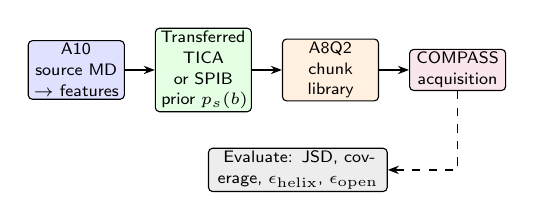
\begin{tikzpicture}[
  font=\sffamily\fontsize{6.5pt}{7.5pt}\selectfont,
  node distance=0.2cm and 0.38cm,
  box/.style={draw, rounded corners=1.5pt, minimum height=0.48cm, text width=11.5mm, align=center, inner sep=1pt},
  arr/.style={-{Stealth[length=1.4mm]}, semithick}
]
\node[box, fill=blue!12] (a10) {A10 source MD\\$\rightarrow$ features};
\node[box, right=of a10, fill=green!10] (lat) {Transferred TICA or SPIB\\prior $p_s(b)$};
\node[box, right=of lat, fill=orange!12] (lib) {A8Q2 chunk library};
\node[box, right=of lib, fill=purple!10] (pol) {COMPASS acquisition};
\node[box, below=0.45cm of lat, xshift=1.2cm, fill=gray!14, text width=22mm] (ev) {Evaluate: JSD, coverage, $\epsilon_{\mathrm{helix}}$, $\epsilon_{\mathrm{open}}$};
\draw[arr] (a10) -- (lat);
\draw[arr] (lat) -- (lib);
\draw[arr] (lib) -- (pol);
\draw[arr, dashed] (pol.south) |- (ev.east);
\end{tikzpicture}%
}
\end{tocentry}

\section{Introduction}

Atomistic molecular dynamics (MD) simulations provide a quantitative bridge between chemical detail and biophysical behavior, but the timescale gap between integrator step and biologically relevant rare events makes naive long-time sampling infeasible for almost all interesting systems.\cite{lindorff2011how,chodera2014markov}
A commodity GPU can produce hundreds of nanoseconds per day for small solvated peptides, but folding, mutational redistribution, and ligand binding routinely demand microsecond-to-millisecond statistics.
Closing this gap is a central methodological challenge of computational chemistry, and it has motivated decades of work on enhanced sampling, Markov state models (MSMs), and adaptive trajectory-generation schemes.\cite{laio2002escaping,barducci2008well,prinz2011markov,husic2018markov,zuckerman2017weighted,huber1996we}

Adaptive sampling reframes the problem as sequential decision-making: rather than running one long trajectory, one launches many short trajectories and uses partial models built from already-collected data to decide where to launch next.
Bowman, Ensign, and Pande introduced MSM-based adaptive sampling that targets uncertainty in slow eigenvalues,\cite{bowman2010adaptive} and Zimmerman and Bowman generalized this to goal-directed property optimization in the FAST framework, which makes the exploration--exploitation trade-off explicit.\cite{zimmerman2015fast}
Reinforcement-learning approaches such as REAP cast collective-variable selection itself as an adaptive policy,\cite{shamsi2018reap,kleiman2022multiagent} while weighted-ensemble methods provide unbiased rate estimates by carefully reweighting replicated trajectories.\cite{huber1996we,zuckerman2017weighted,yang2024werl}
Each of these methods crucially relies on a meaningful low-dimensional coordinate in which to define progress, and the choice of that coordinate has shifted with the rise of machine-learning collective variables.

Linear time-lagged independent component analysis (TICA) extracts maximally autocorrelated coordinates from time-lagged covariances and has become a standard slow-coordinate estimator for MSM construction.\cite{perezhernandez2013tica,schwantes2013improvements,scherer2015pyemma,noe2017collective}
Nonlinear extensions such as time-lagged autoencoders, VAMPnets, RAVE, and the state predictive information bottleneck (SPIB) replace the linear projection with neural-network encoders trained to retain dynamical or state-predictive information.\cite{wehmeyer2018time,mardt2018vampnets,ribeiro2018rave,wang2021spib,tishby2000information}
Coupling such latent representations to adaptive simulation has been demonstrated by DeepDriveMD\cite{lee2019deepdrivemd} and, more recently, by deep-learning-enhanced weighted-ensemble protocols on protein-folding benchmarks.\cite{leung2025dlwe}
A common assumption in these works is that the latent coordinate is trained on data from the same physical system that is then sampled.
The natural next step---and the regime studied here---is whether such latent coordinates can be \emph{transferred} from a related system that is already well-characterized to a less-studied target, and whether the resulting transferred prior is reliable enough to drive acquisition decisions on the target.

Two facts make transfer worth examining carefully.
First, mutational changes in proteins and peptides can drastically reshape kinetics even when the structural ensemble looks superficially similar, so a latent coordinate trained on one sequence is not guaranteed to be globally faithful to a mutant.
Second, adaptive policies driven by an imperfect prior can fail in two qualitatively different ways: they can over-explore irrelevant regions, raising coverage but corrupting equilibrium populations, or they can over-trust a misaligned density, actively biasing observable estimates.
Neither failure is detected by latent-space metrics alone, and neither is reliably caught by a single random baseline.
A controlled benchmark that can disentangle these failure modes is therefore a prerequisite to deploying a transferred-prior adaptive policy on expensive online MD.

This work introduces such a benchmark.
We define \emph{COMPASS}, a retrospective acquisition protocol in which an existing cached A8Q2 mutant peptide trajectory is partitioned into chunks, and an acquisition policy informed by an A10 wild-type prior selects chunks sequentially.
Hydrogen-bond helix and open labels are withheld from the policy and used only for evaluation.
By varying the latent prior (TICA vs.\ SPIB), the budget, the chunk size, and the prior quality (correct, noisy, shuffled, inverted, uniform), we map out when transferred priors help and when they hurt.
The contributions of this work are: (i)~a scoring function that decomposes any transferred-prior acquisition policy into interpretable density, frontier, and trust components; (ii)~quantitative evidence that transferred TICA acts as a useful density and helix-observable prior on A8Q2 even when global TICA-transfer diagnostics are poor; (iii)~quantitative evidence that transferred SPIB acts as a discovery accelerator but a poor equilibrium-density prior; (iv)~prior-corruption controls demonstrating that whether to trust the prior, rather than latent-space novelty alone, is the central design variable; and (v)~a matched-dynamics MSM-emulator benchmark in which COMPASS is compared, at the same transition-budget and lag, against five principled baselines (single-walk ceiling, independent replicas, uniform, min-count, farthest-point) across 5 preset configurations and 50 random repeats, isolating the distinct contributions of the transferred prior and of generic adaptivity.
The remainder of this report introduces the theoretical framework (Section~2), describes the experimental protocol (Section~3), reports the main retrospective results and the MSM-emulator benchmark (Section~4), discusses interpretation and scope (Section~5), and concludes (Section~6).

\section{Theory and Background}

\subsection{Adaptive Sampling as Sequential Acquisition}

We frame any adaptive MD scheme as a sequential acquisition problem on a candidate set $\mathcal{C}$ of structures or trajectory chunks.
At step $t$, given a history $\mathcal{H}_t = \{c_1,\ldots,c_{t-1}\}$ of previously selected candidates and an evaluation metric $\mathcal{M}$, the policy selects $c_t \in \mathcal{C}\setminus\mathcal{H}_t$ to maximize a scoring function $S_t(c)$.
The goal is to reduce the expected loss after adding $c_t$, $\mathbb{E}[\mathcal{M}(\mathcal{H}_t \cup \{c_t\})]$.
In online MD, $\mathcal{C}$ corresponds to candidate restart points and $\mathcal{M}$ measures observable error or distributional accuracy after launching a new trajectory.
In the retrospective benchmark used here, $\mathcal{C}$ is the set of cached chunks from a target trajectory and $\mathcal{M}$ is computed from the union of selected chunk frames.

The retrospective view discards trajectory dynamics during acquisition (no new MD is launched), but it preserves the structure of the decision problem. A policy that performs well retrospectively on a faithful target library is a necessary --- though not sufficient --- condition for performing well online. Conversely, a policy that fails retrospectively is unlikely to recover prospectively, because online MD only adds noise from finite trajectory length.

\subsection{Slow-Coordinate Priors via TICA}

Throughout this work, TICA appears only as a route to a \emph{reference occupancy}: projecting the A10 source trajectory onto a few low-dimensional TICs, histogramming those projections, and reading off bin weights $p_s(b)$. Acquisition then asks which A8Q2 chunks would pull the empirical histogram of selected frames toward that reference---not whether the A10 eigenvectors are a valid global kinetic model of A8Q2 (that empirical question is tested downstream). The standard TICA construction implemented in PyEMMA is as follows.

Time-lagged independent component analysis seeks coordinates $\boldsymbol\chi(\mathbf{x})$ that maximize autocorrelation at lag $\tau$.\cite{perezhernandez2013tica,schwantes2013improvements} For mean-free featurized configurations $\mathbf{x}_t$, the instantaneous and (symmetric) time-lagged covariance matrices are
\begin{equation}
\begin{split}
    \mathbf{C}(0) &= \mathbb{E}_t\!\left[\mathbf{x}_t \mathbf{x}_t^{\top}\right],\\
    \mathbf{C}(\tau) &= \tfrac{1}{2}\mathbb{E}_t\!\left[\mathbf{x}_t \mathbf{x}_{t+\tau}^{\top} + \mathbf{x}_{t+\tau} \mathbf{x}_t^{\top}\right].
\end{split}
    \label{eq:tica_covariances}
\end{equation}
These define the generalized eigenproblem $\mathbf{C}(\tau)\mathbf{u}_i = \lambda_i \mathbf{C}(0)\mathbf{u}_i$, whose top eigenvectors give a linear basis ordered by autocorrelation timescale. The symmetric estimator in Eq.~(\ref{eq:tica_covariances}) is the reversibility-aware choice used by PyEMMA\cite{scherer2015pyemma} and is appropriate for equilibrium peptide ensembles. Histogramming the projections of a source trajectory along the leading TICA components yields bin counts; the implementation adds a uniform pseudo-count of unity per bin, normalizes to obtain $p_s(b)$, then applies any prior-corruption test (Section~\ref{sec:prior_quality}). In the present setting, $p_s$ is computed from the A10 source and used as an observable-aligned prior on A8Q2 chunks projected through the same TICA basis. We make no claim that the transferred basis is a faithful kinetic model on A8Q2; we test whether it is informative as a density prior on A8Q2 sampling decisions.

\subsection{State-Predictive Priors via SPIB}

SPIB training rewards encodings that retain information about a \emph{coarse dynamical label} after lag $\tau$; it does \emph{not} fit an equilibrium density in latent space. Using SPIB coordinates in the same way as a TICA histogram prior therefore risks asking ``where are transitions interesting?'' while assuming the answer coincides with ``where should equilibrium mass live?''---a mismatch we make explicit in the results. The state predictive information bottleneck\cite{wang2021spib} implements this trade-off by jointly training an encoder $q_\phi(\mathbf{z}\mid\mathbf{x})$ and a softmax classifier $p_\theta(y\mid\mathbf{z})$ on configurations $\mathbf{x}$, latent $\mathbf{z}$, and a self-consistent coarse state $y_{t+\tau}$ at lag $\tau$. The standard variational objective is
\begin{equation}
\begin{split}
    \mathcal{L}_{\mathrm{SPIB}}(\phi,\theta) &=
    \mathbb{E}_{q_\phi}\!\left[\log p_\theta(y_{t+\tau}\mid \mathbf{z}_t)\right] \\
    &\quad - \beta\,D_{\mathrm{KL}}\!\left(q_\phi(\mathbf{z}\mid\mathbf{x})\,\Vert\,r(\mathbf{z})\right),
\end{split}
    \label{eq:spib_loss}
\end{equation}
where $\beta>0$ is the information-bottleneck Lagrange multiplier that controls the predictive--compression trade-off and $r(\mathbf{z})$ is a fixed marginal latent prior (a unit isotropic Gaussian throughout this work). Eq.~(\ref{eq:spib_loss}) is the time-lagged generalization of the information-bottleneck principle of Tishby et al.\cite{tishby2000information} to molecular kinetics, with the state assignment refined iteratively until convergence as in the original SPIB algorithm. SPIB latents are nonlinear and tend to emphasize transition-relevant structure rather than equilibrium density. They are therefore well suited to highlight under-explored \emph{regions of dynamical relevance}, and we treat them in this work as discovery coordinates rather than as density estimators.

\subsection{Source-Prior--Deficit Acquisition}
\label{sec:theory_score}

The central idea of COMPASS is a \emph{source-prior--deficit} score. Let $n_t(b)$ be the number of acquisition steps up to $t$ whose \emph{decision bin} is $b$: in retrospective replay, the bin of the chunk \emph{start} frame; in the MSM emulator, the bin of the restart microstate. The implementation sets $\hat{p}_t(b)=n_t(b)/\sum_{b'} n_t(b')$ from these counts only---not from pooling every frame inside already-selected chunks (Section~\ref{sec:methods_compass}). Relative to $p_s(b)$, the policy rewards candidates that shrink bins where source-supported mass is still under-represented under those start-bin statistics. The equations below make that comparison stable when a few high-$p_s$ bins would otherwise dominate, and combine the resulting signal with frontier and trust terms into a single scalar score (Eq.~\ref{eq:score}). The raw deficit
\begin{equation}
    d_t(b) = \max\!\left[p_s(b) - \hat{p}_t(b),\,0\right]
    \label{eq:raw_deficit}
\end{equation}
flags bins where source-supported mass is currently under-represented in the selected sample. However, the raw deficit scales linearly with $p_s$ and saturates slowly at high-density bins, so a few dominant bins can monopolize the score. We therefore use an information-gain form
\begin{equation}
\begin{split}
    d^{IG}_t(b) &= \frac{N_t(b)}{1+\lambda\,p_s(b)},\\
    N_t(b) &= p_s(b)\,\max\!\left[1-\frac{\hat{p}_t(b)}{\max(p_s(b),10^{-12})},\,0\right].
\end{split}
    \label{eq:ig_deficit}
\end{equation}
Here $N_t(b)$ measures source mass in bin $b$ scaled by fractional under-filling relative to $\hat{p}_t$, and the denominator $1+\lambda p_s(b)$ down-weights heavily populated bins once they are partially filled; $\lambda\geq 0$ controls how aggressively common bins are de-emphasized, and $\lambda=20$ is fixed in code (Section~\ref{sec:methods_compass}). The acquisition score first forms a weighted sum of $K$ min--max standardized components (source deficit, representativeness, boundary trust, frontier disagreement, unvisited factor, distance novelty, and redundancy) with weights $w_k(t)$ from the phase scheduler (Table~\ref{tab:policy_weights}), then multiplies by a \emph{bin fatigue} factor tied to how often the candidate's bin has already been chosen:
\begin{equation}
    S_t(c) = \frac{1}{1+n_{b(c)}}\sum_{k=1}^{K} w_k(t)\,z_k(c),
    \label{eq:score}
\end{equation}
where $b(c)$ is the candidate's decision bin (chunk-start bin in replay, restart bin in MSM), $n_{b(c)}$ is the corresponding count $n_t(b(c))$ \emph{before} adding step $t$, each $z_k(c)$ lies in $[0,1]$ after per-step min--max scaling over remaining candidates, and the \emph{redundancy} component uses $z_{\mathrm{red}}(c)=\exp(-d_{\min}^2(c)/\kappa)$ with $d_{\min}(c)$ the Euclidean distance in the latent used for frontier scoring to the nearest prior decision point and $\kappa=0.02$ in latent units squared.

The decomposition has a useful practical consequence. The density terms $\{d_t,d^{IG}_t,\text{representativeness}\}$ are tied to the source prior and degrade gracefully only if the prior is approximately correct. The frontier and novelty terms are prior-independent and continue to drive exploration even when the prior is misleading. Negative weight on redundancy penalizes near-duplicates in latent space, while the prefactor $1/(1+n_b)$ additionally damps repeated picks that land in the same bin; trust weights modulate prior versus exploratory terms. Failures of a transferred prior can therefore be attributed to specific terms rather than to ``adaptive sampling'' as a monolithic black box. This identifiability is what makes the framework useful as a diagnostic before online deployment.

\section{Methodology}

\subsection{Study Design and Scope}

We studied adaptive acquisition for the A8Q2 mutant peptide using a retrospective replay protocol. In this setting, no new molecular dynamics (MD) trajectories are launched during the benchmark. Instead, an existing A8Q2 trajectory library is partitioned into fixed-length chunks, and an acquisition policy selects a subset of those chunks in sequence. The retrospective setting is intentionally conservative for method development: it enables controlled comparisons across policies and random baselines, but it does not by itself establish online wall-clock acceleration.

All improvements reported below should therefore be interpreted as acquisition-policy improvements within a fixed precomputed target library. They do not establish unbiased kinetics, equilibrium reweighting, or prospective acceleration of MD. The benchmark is intended to answer a narrower question that is useful before online deployment: would a transferred prior have selected informative chunks from the target library?

Retrospective COMPASS and its bootstrap-random baseline both draw candidate chunks from the \emph{complete} cached target library: every trajectory frame is admissible in principle. That shared action set is an \emph{oracle} relative to true online MD, where only states already produced by launched simulations may be restarted. Headline margins against random should therefore be read as diagnostics on a fixed library, not as certified online wall-clock gains. The MSM-emulator benchmark in Section~\ref{sec:methods_msm} is the complementary, \emph{online-faithful} abstraction within Markov dynamics alone: restarts are restricted to microstates visited along simulated walks, mirroring how online MD may only re-seed from states already visited in prior segments.

The central scientific question is whether information learned from the wild-type A10 peptide can guide sampling of A8Q2. The transferred information was restricted to generic torsional features projected through learned latent maps. Helix/open labels derived from native hydrogen bonds were used only after acquisition for evaluation. This separation was used to avoid directly optimizing the same observables used to judge the policy.

\subsection{Computational Details}

\paragraph{Molecular dynamics.}
The A10 source and A8Q2 target reference trajectories were generated with \textsc{OpenMM}~8\cite{eastman2024openmm8} using explicit solvent, the additive CHARMM36m force field with CHARMM-modified TIP3P water (\textsc{OpenMM} \path{charmm36_2024} files),\cite{huang2017charmm36m,kim2015charmmgui} electrostatics treated by particle-mesh Ewald, a 1.2~nm nonbonded cutoff with 1.0--1.2~nm switching, hydrogen--heavy-atom and rigid-water constraints, a 2~fs timestep, and a Langevin middle integrator (friction 1~ps$^{-1}$).
After minimization and equilibration (NVT with peptide restraints, then NPT as detailed in the Supporting Information), production NVT simulations were run at \textbf{330~K} for both peptides so that helix--coil statistics are sampled efficiently on a laboratory-accessible budget while keeping the A10/A8Q2 comparison internally consistent.
Coordinates were saved every 0.1~ns (100~ps) for featurization and chunk construction.

\paragraph{Models and replay.}
TICA was fit on backbone torsional features using PyEMMA's symmetric covariance estimator;\cite{scherer2015pyemma} SPIB encoders were trained with PyTorch on the same A10 source features.
Helix and open evaluation used native hydrogen-bond counts with an extended helical definition of $N_{\mathrm{HB}}\geq 3$ and an open definition of $N_{\mathrm{HB}}\leq 1$ (\texttt{DEFAULT\_HELIX\_NHB\_THRESHOLD} / \texttt{DEFAULT\_OPEN\_NHB\_THRESHOLD} in \path{replay_enhanced.py}), consistent with the analysis header in \path{src/analysis.py}.
Acquisition scoring, replay execution, and metric evaluation were implemented in Python; code paths are \path{src/compass/replay_enhanced.py} and \path{scripts/compass_experiments_enhanced.py}.
\textbf{Follow-on code (COMPASS v2):} \path{src/compass/v2/bench.py} replaces full-library oracle chunk replay with causal archive playback plus an equivalence-cloud candidate generator (oracle-only RMSD/Torsion/Target-TICA/Macrostates); see \path{COMPASS_PLAN.md} \S1.2 and \path{docs/COMPASS_V2_REPRODUCTION.md}.
The Supporting Information file \path{paper/COMPASS_JCTC_SUPPORTING_INFORMATION.pdf} lists the full MD checklist, training notes, and a complete table of sweep metrics for all replay experiments.

\subsection{Transferred Latent Atlases}

\subsubsection{TICA Atlas}
\label{sec:tica_atlas}

A10-fitted TICA supplied the mean vector and projection matrix; A10 and A8Q2 features were projected into the same TICA space and the first two coordinates defined a two-dimensional source-density grid. \emph{Reported experiments} build bin edges from the \textbf{source} trajectory only: for each axis, the 0.5--99.5 percentile range on the source projection is padded by 8\% of its width and split into $n_x$ (and, for 2D maps, $n_y$) equal-width cells (\texttt{bin\_edges\_mode=source\_only}, default in \path{replay_enhanced.py} and in \path{compare_msm_three_policies.py}). A \texttt{pooled} pooling mode (joint source--target percentiles) exists but was not used for the results here. In a prospective setting, the same source-only rule is the reproducible choice when the target is unknown; replay used a fixed grid for evaluation.

Formal A10$\rightarrow$A8Q2 transfer scores ($D_0$, $D_{\tau}$, $D_{KM}$) read as poor-to-marginal global fidelity, yet leading TIC directions still overlap the native A8Q2 subspace and transferred TIC-1 stays strongly helix-correlated (Fig.~\ref{fig:transfer}). We therefore use A10 TICA here as an empirical 2-D density and observable prior on A8Q2, not as a certified A8Q2 kinetic model. The residual slow structure (notably a Gln-localized backbone-$\phi$ mode absent from the homopolymer source) motivates treating MSM-bin coarse-graining as blind to that degree of freedom in Section~\ref{sec:methods_msm}.

\subsubsection{SPIB Atlas}

A10-trained SPIB encoders projected A8Q2 features into either one- or two-dimensional SPIB latent coordinates.\cite{wang2021spib} Because the encoder was also transferred and not retrained on A8Q2, SPIB results are interpreted as tests of discovery behavior rather than as direct estimates of equilibrium thermodynamics on the target.

\subsection{Trajectory Chunk Library}

The target A8Q2 trajectory was partitioned into non-overlapping chunks of length $L$ frames. With a frame spacing of $0.1$\,ns, the main $80$\,ns TICA and SPIB experiments used $L=10$ ($T_c=1$\,ns chunks), the short-budget observable experiment used $L=20$ ($T_c=2$\,ns chunks), and the long-budget TICA experiment selected 200 chunks for a total acquired time of $200$\,ns. At each acquisition step the policy selected one previously-unselected chunk; the union of selected frames was used to compute all latent-space and observable metrics.

\subsection{COMPASS Acquisition Policy}
\label{sec:methods_compass}

The acquisition score follows the source-prior--deficit decomposition introduced in Section~\ref{sec:theory_score} (Eqs.~\ref{eq:raw_deficit}--\ref{eq:score}). For each latent atlas, source histogram counts receive a unit pseudo-count per bin, normalizing to $p_s(b)$; prior-corruption experiments replace $p_s$ after smoothing. \textbf{Scoring} compares $p_s$ to $\hat{p}_t$ from the empirical distribution of \emph{decision bins}---chunk-start bins in replay, restart bins for B6 in the MSM runner---whereas reported JSD, coverage, and observables aggregate \textbf{all frames} from selected chunks (replay) or lag-weighted MSM mass (emulator). Most experiments used the information-gain deficit (Eq.~\ref{eq:ig_deficit}) with $\lambda=20$. The seven weighted components are the Table~\ref{tab:policy_weights} rows; their $z_k$ constructions min--max scale over feasible candidates at each step as summarized in Section~\ref{sec:theory_score}. Unless otherwise stated, the selected chunk was the highest-scoring remaining chunk; stochastic confirmation experiments used a temperature softmax over the top five candidates (\texttt{top\_k=5} in \path{src/compass/replay_enhanced.py}).

The component weights $w_k(t)$ followed a two-phase schedule (Table~\ref{tab:policy_weights}): exploratory and boundary terms dominated the first $30\%$ of the budget, balanced terms governed the middle $40\%$, and source-density correction dominated the final $30\%$. The schedule was designed to separate two objectives that often conflict: discovering source-supported regions and estimating equilibrium-like target observables. For TICA and SPIB maps in this work, all density, frontier, and novelty quantities were evaluated in the same single-latent space; controlled hybrid scoring is deferred to the online setting where an explicit trust controller can be applied.

\begin{table}[htbp]
    \centering
    \caption{Weights $w_k(t)$ used by the non-hybrid two-phase scheduler. The first 30\% of the budget used exploratory weights, the middle 40\% used balanced weights, and the final 30\% used exploit weights. The redundancy row is negative and drives a latent-space proximity penalty (Eq.~\ref{eq:score}); an additional bin fatigue prefactor $1/(1+n_b)$ scales the entire linear combination.}
    \label{tab:policy_weights}
    \small
    \setlength{\tabcolsep}{3.5pt}
    \begin{tabular}{@{}lrrr@{}}
        \toprule
        Component $z_k$ & Expl. & Bal. & Exploit \\
        \midrule
        Source deficit ($d^{IG}_t$) & 0.15 & 1.25 & 1.45 \\
        Source representative & 0.10 & 0.65 & 0.85 \\
        Source-boundary trust & 1.20 & 0.25 & 0.15 \\
        Frontier disagreement & 0.90 & 0.35 & 0.10 \\
        Unvisited & 0.75 & 0.25 & 0.15 \\
        Novelty & 0.65 & 0.25 & 0.10 \\
        Redundancy & $-0.90$ & $-0.80$ & $-0.60$ \\
        \bottomrule
    \end{tabular}
\end{table}

\begin{figure*}[htbp]
    \centering
    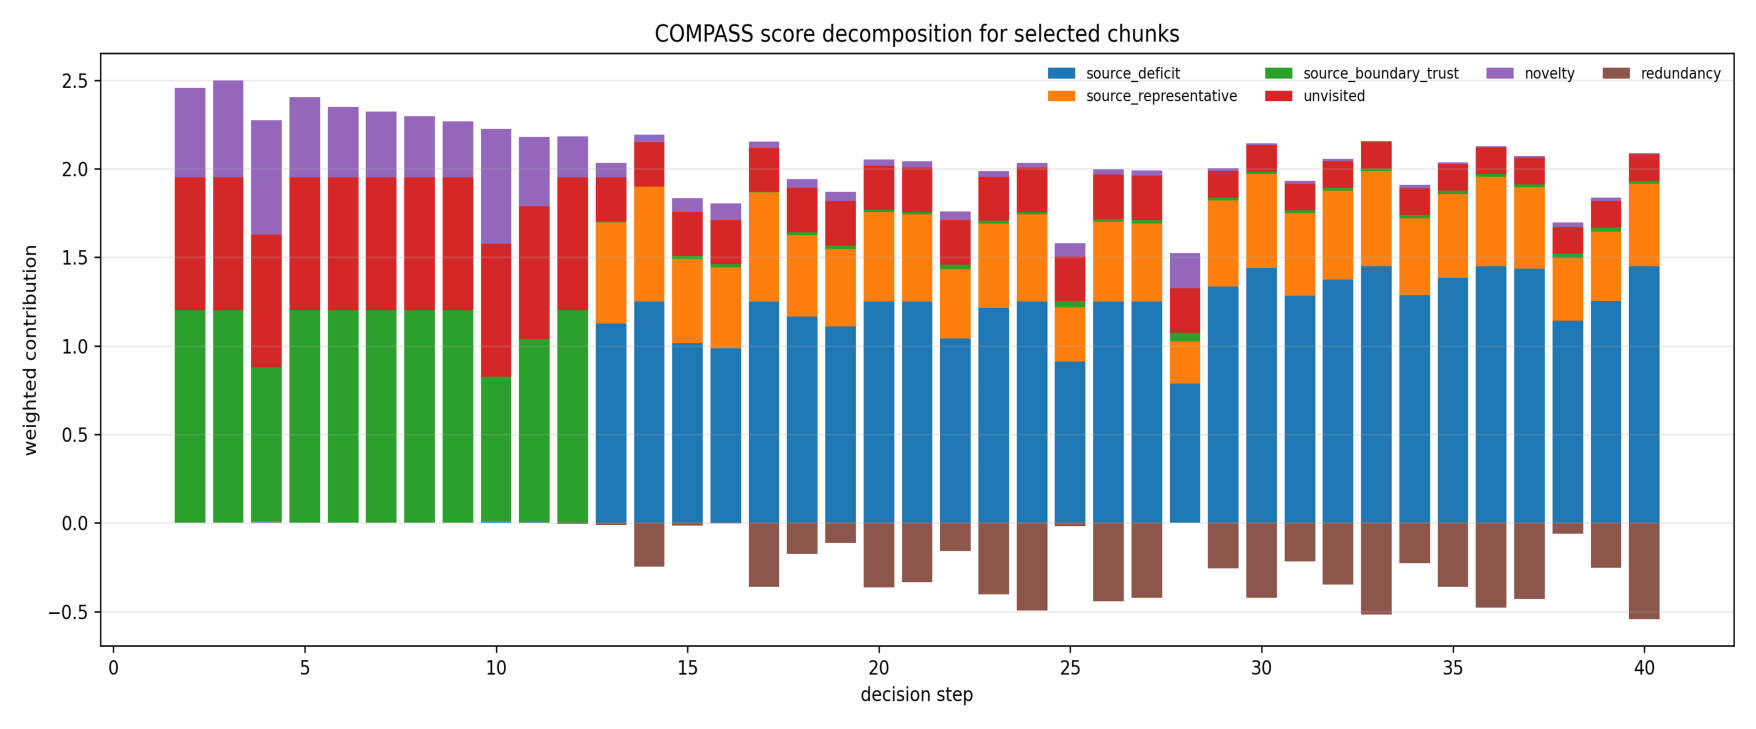
\includegraphics[width=0.92\linewidth]{score_decomposition_e12.png}
    \caption{Score-component decomposition for the main TICA2D two-phase acquisition ($T_c=2$\,ns chunks, $80$\,ns budget, 40 steps). Each stacked bar shows the weighted contribution of each scoring component for the selected chunk at that step. The phase transition is visible: early steps (1--12, exploratory phase) are dominated by source-boundary trust (green) and unvisited-bin preference (red); later steps (29--40, exploit phase) are dominated by source deficit (blue) and representativeness (orange). Negative bars (brown) show the redundancy penalty. This decomposition makes the policy's decision process interpretable at each acquisition step.}
    \label{fig:score_decomp}
\end{figure*}

\subsection{Baselines and Evaluation Metrics}

The main baseline was bootstrap random acquisition. For each random repeat, chunks were drawn with replacement from the same target chunk library, and the same cumulative metrics were computed. Reported random means and uncertainty bands used 100 random repeats. This baseline is strong because it samples from the completed A8Q2 library rather than from a degraded model of target dynamics; failures against random are therefore meaningful. It is also not identical to the no-replacement deterministic COMPASS selection rule, so the bootstrap baseline is interpreted as an uncertainty envelope rather than as the only possible random comparator.

The primary distributional metric was Jensen--Shannon divergence (JSD) between the selected and reference two-dimensional histograms, restricted to reference bins whose \textbf{raw} frame count is at least three (\texttt{min\_count=3} in \path{replay_enhanced.py}), then symmetrically normalized on that mask. Coverage was the fraction of those same reference-supported bins visited by the selected sample. Important coverage used bins with the largest smoothed source probabilities: the top $k$ cells, with $k=\min\{\max(20,\lfloor B/20\rfloor),B\}$ for $B$ total bins (\texttt{\_important\_source\_mask} in \path{src/compass/replay_enhanced.py}), matching the emulator's first-passage bookkeeping. Source mass visited was $\sum_{b:\,\mathrm{visited}} p_s(b)$ over that smoothed prior.

Observable metrics were computed from hydrogen-bond labels after selection. The helix fraction \(f_{\mathrm{helix}}\) and open fraction \(f_{\mathrm{open}}\) were compared with full-target reference values (superscript $\text{sel}$ denotes the selected-sample estimate):
\begin{equation}
\begin{split}
    \epsilon_{\mathrm{helix}} &= \bigl| f_{\mathrm{helix}}^{\text{sel}} - f_{\mathrm{helix}}^{\mathrm{ref}} \bigr|,\\
    \epsilon_{\mathrm{open}} &= \bigl| f_{\mathrm{open}}^{\text{sel}} - f_{\mathrm{open}}^{\mathrm{ref}} \bigr|.
\end{split}
\end{equation}
These labels were not available to the acquisition policy. They were used only to test whether latent-space acquisition preserved physically interpretable populations.

\subsection{Selected Experiments}

The full sweep included static policies, annealed policies, prior-corruption tests, SPIB variants, and stochastic repeats. The experiments presented here are those that support a coherent mechanistic story:
\begin{enumerate}
    \item TICA2D two-phase acquisition with \SI{2}{ns} chunks at \SI{80}{ns}, testing short-budget observable estimation.
    \item SPIB1D two-phase acquisition at \SI{80}{ns}, testing discovery and source-mass coverage.
    \item TICA2D two-phase acquisition at \SI{200}{ns}, testing long-budget distributional recovery.
    \item Uniform, shuffled, noisy, and inverted TICA priors, testing whether prior quality controls failure modes.
\end{enumerate}
Stochastic-start variants and pure-frontier ablations are reported in the Supporting Information; the prior-corruption tests above already isolate the failure modes (over-trust of a misaligned density, exploration without density correction) that those auxiliary runs would otherwise demonstrate.

\subsection{Matched-Dynamics MSM-Emulator Benchmark}
\label{sec:methods_msm}

The retrospective replay above answers ``would a transferred prior have selected informative chunks from the cached target library?'', but its single baseline is \emph{bootstrap random} over a finite cached library. It cannot, by itself, separate two distinct contributions to any observed COMPASS gain: the value of the transferred prior, and the generic value of adapting the restart distribution as data accrues. To disentangle these, and to produce policy comparisons that are cleanly apples-to-apples (same dynamics, same lag, same bins, same random seeds), we introduce a second, orthogonal benchmark.

\paragraph{MSM emulator.} Policies are compared under identical Markov dynamics: one row-stochastic transition matrix $\mathbf{T}$ is estimated on the full A8Q2 target trajectory using the same atlas bins and lag $\tau$ used by COMPASS at each preset; the only quantity that varies across methods is the rule that picks each restart microstate. Rather than launching new MD, each policy at round $t$ chooses a restart microstate $s^{\mathrm{start}}_t$ and simulates a short Markov walk $s_0=s^{\mathrm{start}}_t \to s_1 \to \ldots \to s_{n}$ of $n$ transitions under that shared $\mathbf{T}$. Each state along the walk contributes a lag-weighted mass $\tau\cdot\Delta t_{\mathrm{frame}}$ ($=1$\,ns for $\tau=10$ frames at the 0.1\,ns frame spacing used throughout) to the cumulative histogram on the bin grid, from which all metrics --- JSD, coverage, $|\Delta f_{\mathrm{helix}}|$, $|\Delta f_{\mathrm{open}}|$ --- are computed at every round. All policies share the same initial microstates (cycled over the same preset seed list), the same total transition budget, and the same random-number stream across repeats wherever the policy is deterministic. Results are averaged over 50 independent stochastic repeats per preset, and the JSD noise floor is estimated by 200 two-half bootstrap splits of the target trajectory (median, 95th percentile).

\paragraph{Observable evaluation.} JSD measures only how simulated mass is distributed across latent bins, whereas helix and open errors measure how the resulting mass-weighted mixture of bin-local compositions matches the global target fractions; improving one does not imply improving the other. Concretely, helix and open fractions in the emulator are \emph{not} recomputed by threading raw MD frames through each new walk. After each round, $f_{\mathrm{helix}}$ and $f_{\mathrm{open}}$ are the histogram-weighted averages of per-microstate fractions $f_{\mathrm{helix}}(s)$, $f_{\mathrm{open}}(s)$ obtained by binning the full target trajectory (the \texttt{microstate\_observables} construction in the companion code). Policies that steer mass into bins with extreme local helix/open composition---for example pure min-count or geometric novelty rules on a coarse 1D grid---can therefore corrupt observables even while partially improving latent coverage.

\paragraph{Baselines.} Six policies are benchmarked under the identical emulator:
\begin{description}
    \item[B0 --- single-walk ceiling.] One continuous Markov walk of length $N_{\mathrm{walks}}\times N_{\mathrm{steps}}$ transitions, sliced into $N_{\mathrm{walks}}$ equal-length segments so a per-round curve exists. This is a diagnostic upper bound: it pays zero restart cost under Markov dynamics and is therefore optimistic relative to real MD.
    \item[B1 --- independent replicas.] $N_{\mathrm{walks}}$ separate walks launched from fixed initial seeds, no adaptivity. This isolates ``parallel short MD'' with no feedback.
    \item[B2 --- uniform.] Each restart drawn uniformly at random from microstates observed so far.
    \item[B3 --- min-count.] Each restart is the observed microstate with smallest accumulated lag-weighted mass (count-based adaptive, classical FAST-style exploitation of under-sampled states).\cite{zimmerman2015fast}
    \item[B4 --- farthest-point.] Each restart maximizes Euclidean distance between latent \emph{bin centers} from the centroid of prior B4 restarts (on SPIB1D the grid is $30\times1$, so the rule reduces to 1D separation; pure geometric novelty, no prior).
    \item[B6 --- COMPASS.] The full source-prior--deficit score of Eq.~(\ref{eq:score}) with the two-phase schedule of Table~\ref{tab:policy_weights} and the same transferred prior used in the retrospective benchmark.
\end{description}
\noindent An optional seventh identifier, B5 (COMPASS with frontier-only scoring, no density weighting), exists in the software but is not included in the default six-policy ensemble reported here.

\paragraph{Presets.} Five preset configurations span the latent spaces and budgets used in the retrospective benchmark: (1) tICA2D baseline (80 rounds, 10 frames/chunk, 1 seed, 160\,ns total), (2) tICA2D long-chunk (40 rounds, 20 frames/chunk), (3) SPIB1D (80 rounds, 10 frames/chunk), (4) tICA2D long-budget (200 rounds, 10 frames/chunk, 400\,ns total), and (5) tICA2D two-seed. Each preset uses its own $\mathbf{T}$, bin grid, and reference histogram. This benchmark therefore controls the dynamics so that policy differences can be attributed cleanly to the acquisition rule, at the cost of inheriting the MSM's coarse-graining: slow modes not exposed by the bin discretization, such as the Gln-localized backbone-$\phi$ mode discussed in Section~\ref{sec:tica_atlas}, are invisible to \emph{every} policy here. Runner: \path{scripts/compare_msm_three_policies.py}; plotting: \path{scripts/plot_msm_benchmark.py}.

\section{Results}

We first relate transfer diagnostics to acquisition outcomes on the real A8Q2 library (TICA and SPIB), then stress-test prior quality, and finally report the MSM-emulator comparison where dynamics are fixed and only restart rules differ.

\subsection{Transferred TICA Is Not Globally Valid but Remains Helix-Informative}

Figure~\ref{fig:transfer} collects the A10$\rightarrow$A8Q2 transfer diagnostics already summarized in Section~\ref{sec:tica_atlas}: formal geometric and kinetic scores indicate a rotated, not faithful, basis, yet leading directions overlap enough that transferred TIC-1 remains strongly helix-correlated. The acquisition experiments below therefore test whether that residual signal is useful for chunk selection rather than whether A10 TICA defines an A8Q2 reaction coordinate.

\begin{figure*}[htbp]
    \centering
    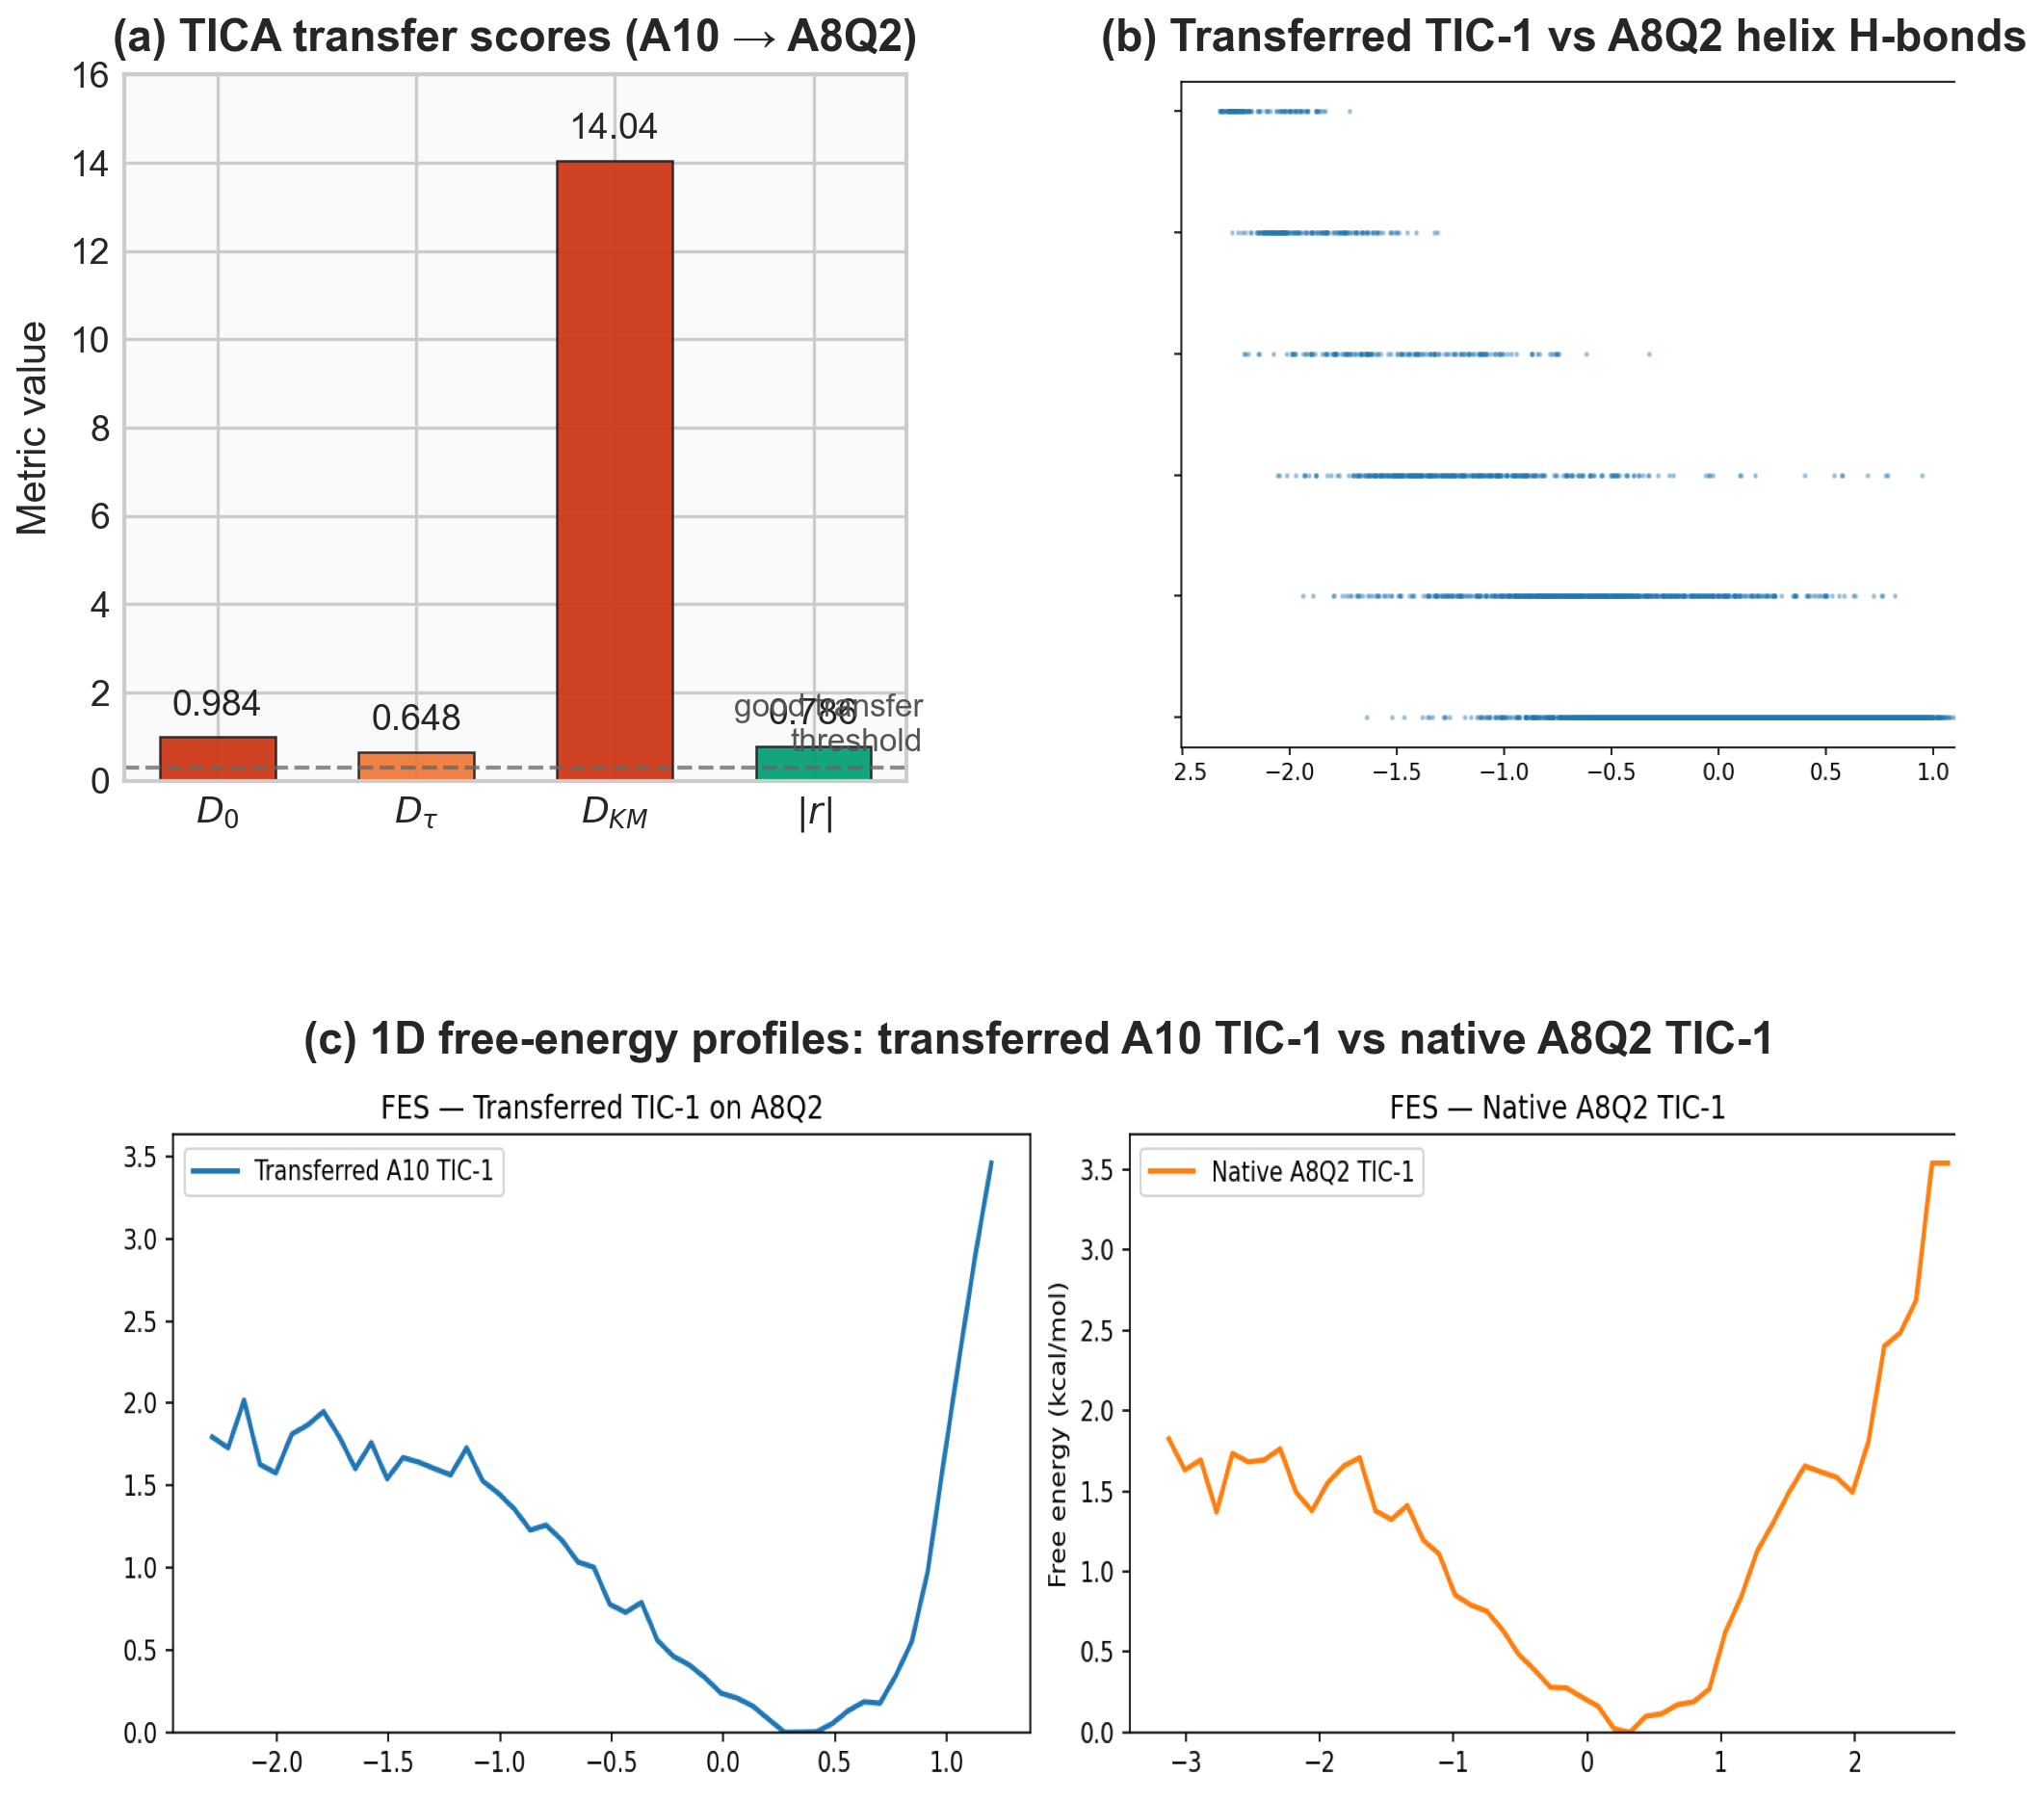
\includegraphics[width=0.92\linewidth]{transfer_diagnostics.png}
    \caption{TICA transfer diagnostics from A10 to A8Q2. (a)~Four transfer metrics (axis labels give definitions): $D_0$ and $D_{KM}$ lie in the poor regime relative to the dashed criteria, $D_\tau$ is marginal, and the absolute correlation $|r|$ between transferred TIC-1 and A8Q2 helix content meets the success threshold. The headline is therefore failed global transfer with a retained helix-direction signal. (b)~Scatter plot of transferred TIC-1 versus A8Q2 hydrogen-bond count $N_{\mathrm{HB}}$, confirming the negative correlation: more negative TIC-1 corresponds to higher helicity. (c)~One-dimensional free-energy profiles along the transferred A10 TIC-1 (left, blue) and along native A8Q2 TIC-1 (right, orange), illustrating why the scalar metrics in (a) read as poor transfer even though a useful helix trend remains.}
    \label{fig:transfer}
\end{figure*}

\subsection{TICA2D Gives a Low Short-Budget Helix Error}

The clearest $80$\,ns observable result was obtained with TICA2D two-phase acquisition using $T_c=2$\,ns chunks. COMPASS selected 40 chunks and achieved a helix-fraction error of $\epsilon_{\mathrm{helix}}=7.5\times 10^{-4}$, compared with $2.08\times 10^{-2}$ for bootstrap random acquisition --- a 28-fold reduction in the absolute deviation from the full-target reference. The open-fraction error also improved, from $\epsilon_{\mathrm{open}}=3.09\times 10^{-2}$ (random) to $2.04\times 10^{-2}$ (COMPASS). Important source-bin coverage was complete for COMPASS (1.000) and essentially complete for random ($0.992$).

This improvement did \emph{not} coincide with better global distributional metrics. The same run had a worse final TICA-space JSD than random ($0.156$ vs.\ $0.139$) and lower raw bin coverage ($0.514$ vs.\ $0.572$). The short-budget result is therefore not a generic ``COMPASS beats random'' claim. It is a targeted result: transferred TICA density guidance recovers a helix-relevant observable under limited budget, while bootstrap random remains stronger for broad target-distribution coverage.

\begin{figure*}[htbp]
    \centering
    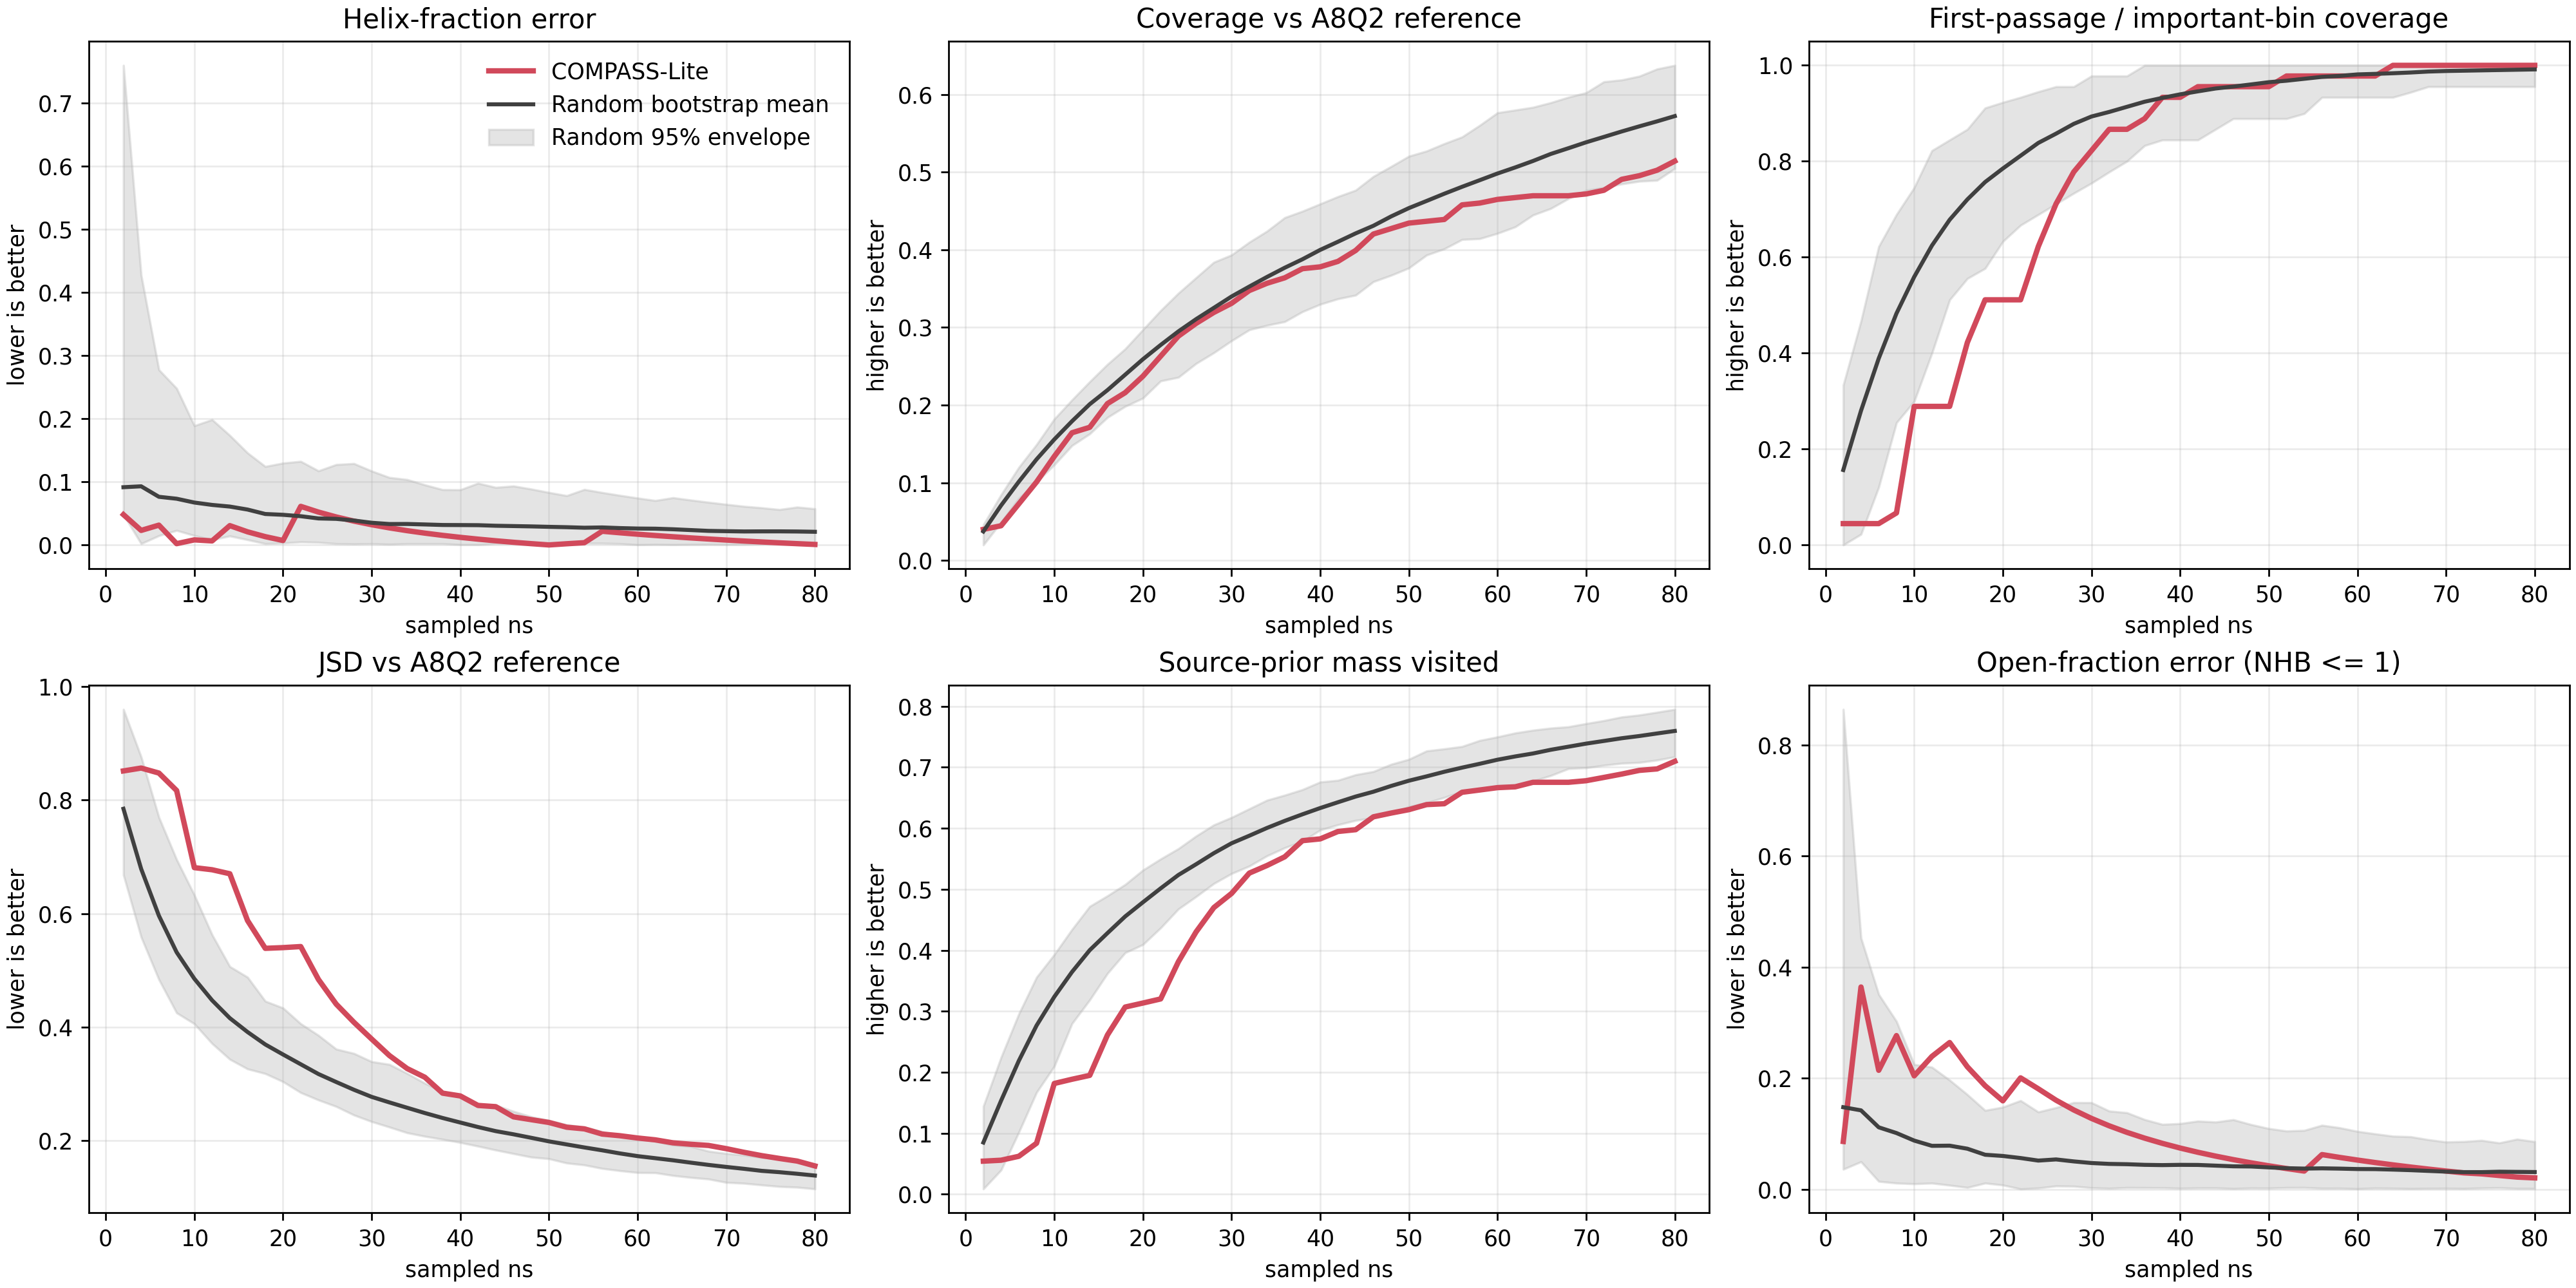
\includegraphics[width=0.92\linewidth]{replay_tica2d_chunk20_80ns.png}
    \caption{Short-budget TICA2D acquisition with $T_c=2$\,ns chunks ($80$\,ns total acquired time, 40 chunks). Cumulative metrics versus selected fraction of budget for COMPASS (solid) and bootstrap random (mean $\pm$ shaded band over 100 repeats). Panels show, from top-left to bottom-right: helix-fraction error $\epsilon_{\mathrm{helix}}$, open-fraction error $\epsilon_{\mathrm{open}}$, TICA-space JSD against the full-target reference, and raw bin coverage. COMPASS gives the lowest observed helix-fraction error of any main $80$\,ns experiment in this study, while random remains competitive or better for global JSD and raw coverage.}
    \label{fig:tica80}
\end{figure*}

\subsection{SPIB1D Accelerates Discovery but Not Equilibrium Estimation}

SPIB1D produced the strongest discovery behavior. At $80$\,ns, SPIB1D two-phase acquisition saturated all three SPIB-space discovery metrics --- raw coverage, important-bin coverage, and source-mass visitation all reached $1.000$ --- compared with random means of $0.863$, $0.963$, and $0.989$ respectively.

The same run, however, performed poorly on helix and open observables. The helix-fraction error was $\epsilon_{\mathrm{helix}}=8.33\times 10^{-2}$ for COMPASS compared with $1.71\times 10^{-2}$ for random---an almost fivefold inflation. The open-fraction error was $7.79\times 10^{-2}$ vs.\ $2.35\times 10^{-2}$ for random. JSD in the SPIB map was also worse than random ($0.014$ vs.\ $0.009$). This cleanly separates two roles that are often conflated in adaptive sampling: a transferred latent coordinate may be excellent for discovering distinct regions while being unsuitable as an equilibrium-density prior.

\begin{figure*}[htbp]
    \centering
    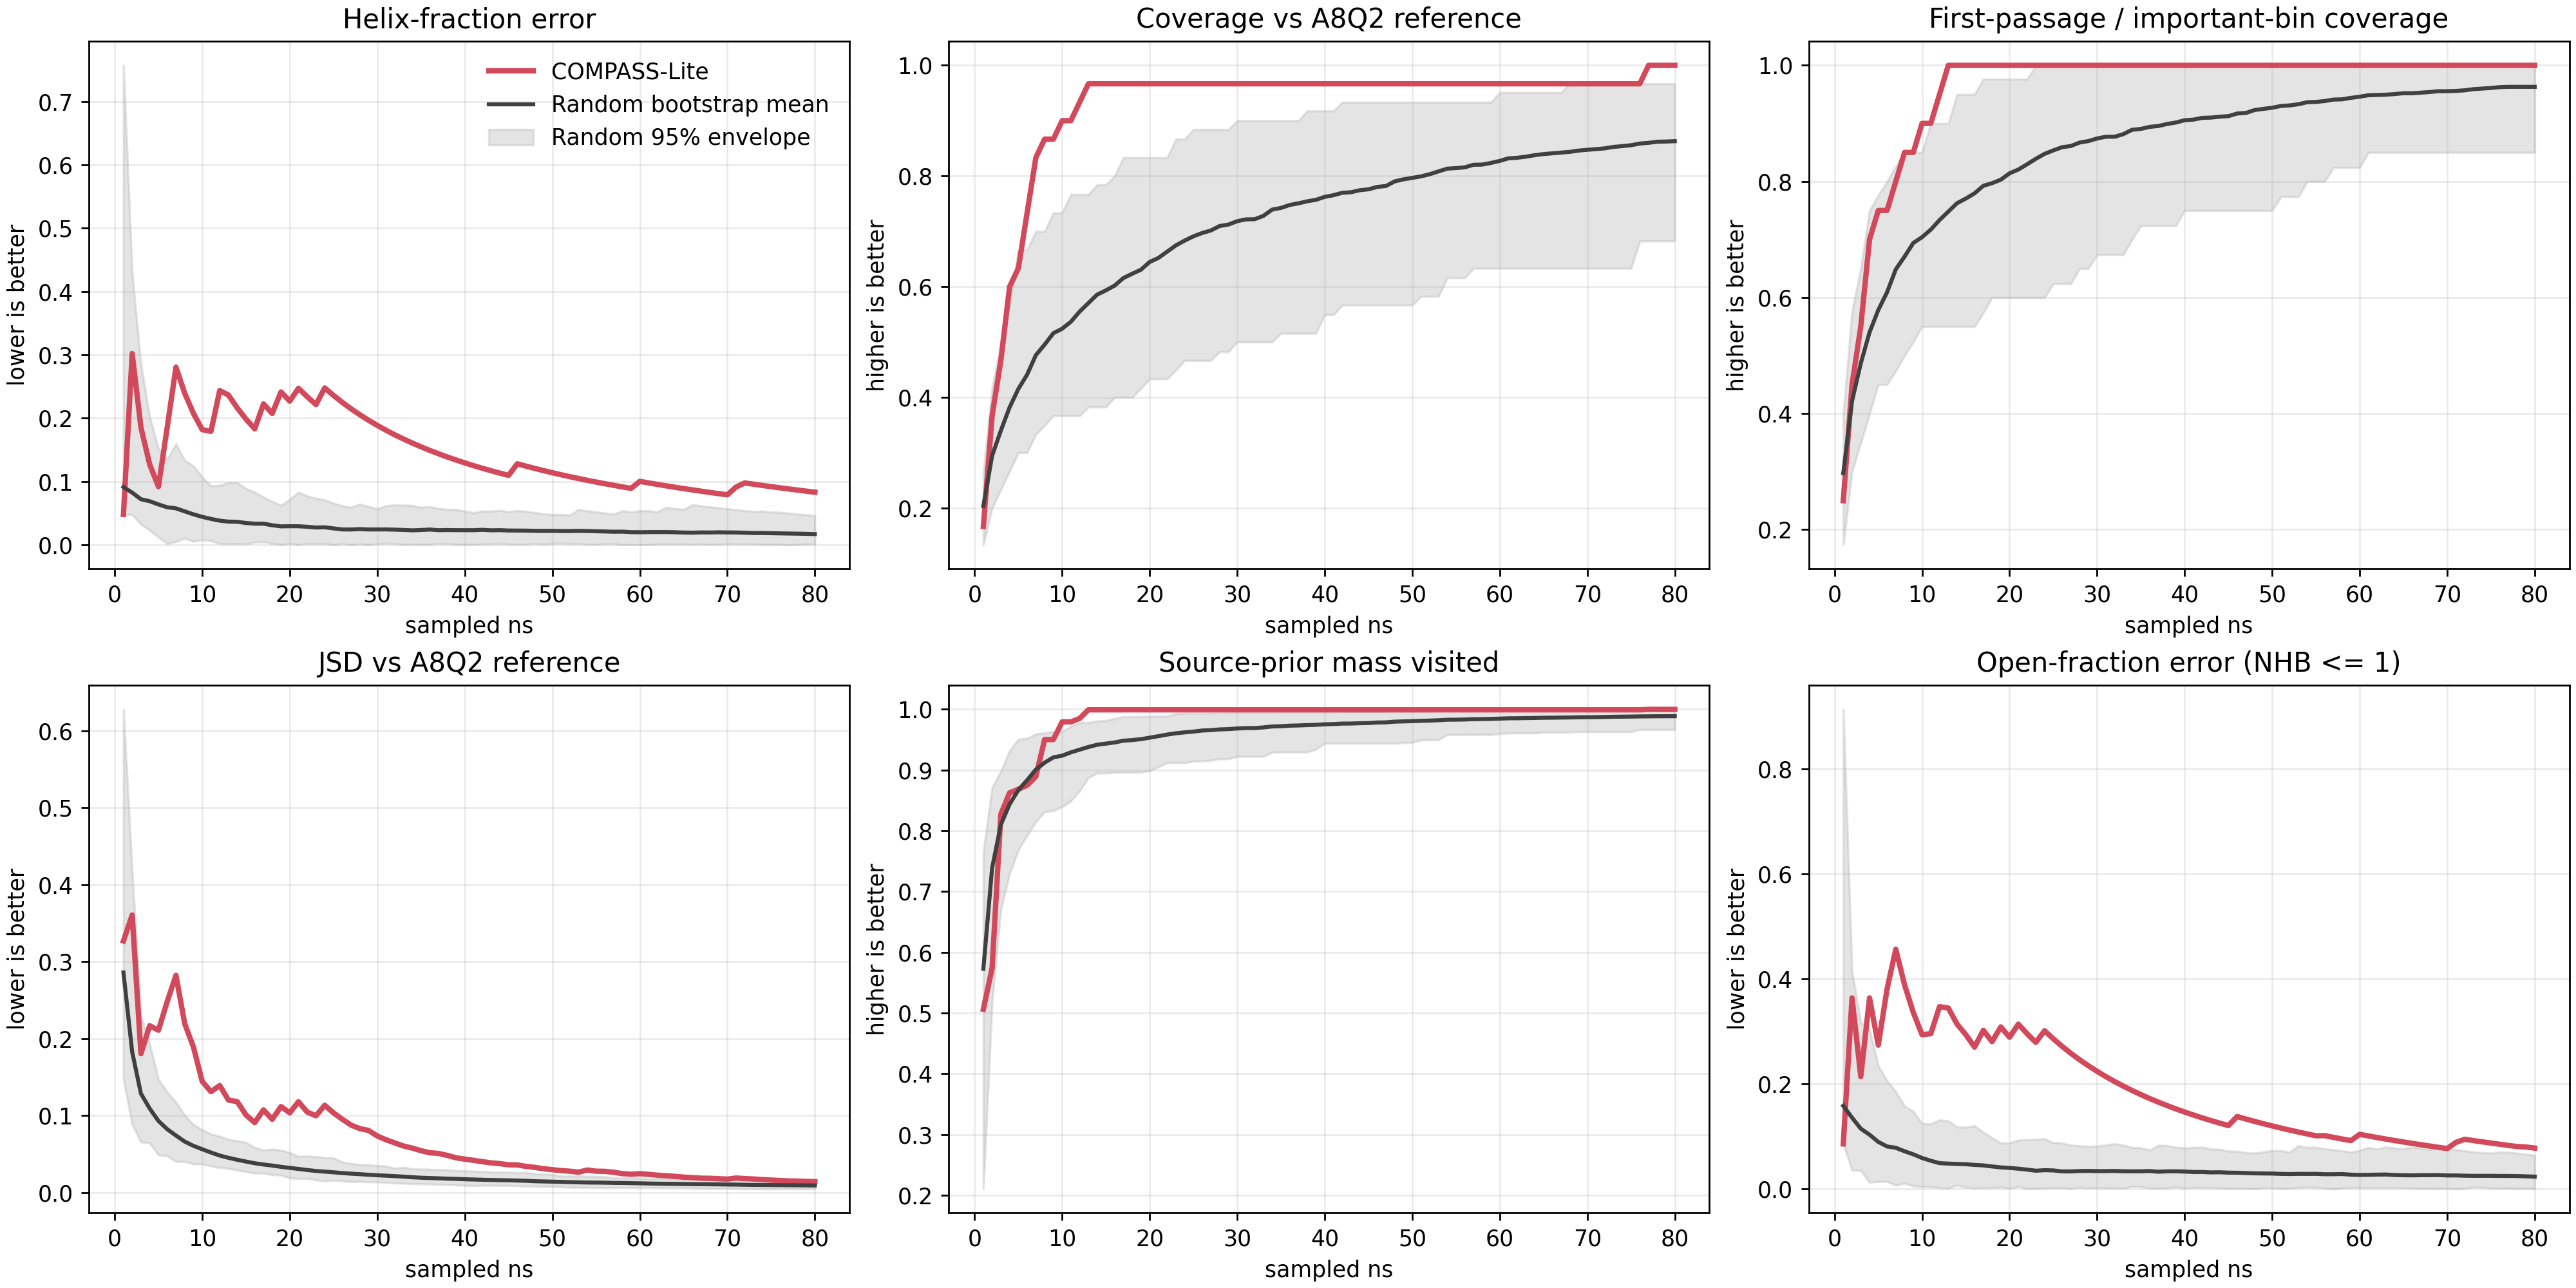
\includegraphics[width=0.92\linewidth]{replay_spib1d_80ns.png}
    \caption{SPIB1D acquisition at $80$\,ns ($T_c=1$\,ns chunks). Curves and bands as in Fig.~\ref{fig:tica80} but with SPIB-space metrics. SPIB1D rapidly saturates source-supported latent coverage but substantially worsens helix/open population estimates, indicating that the transferred SPIB latent should be treated as a discovery coordinate rather than as a density prior.}
    \label{fig:spib80}
\end{figure*}

\subsection{TICA2D Improves Long-Budget Distributional Recovery}

At a $200$\,ns budget, TICA2D two-phase acquisition improved both global JSD and coverage relative to random. COMPASS achieved JSD $0.042$ vs $0.057$ for random, raw coverage $0.880$ vs $0.801$, and source mass visited $0.911$ vs $0.875$. Important-bin coverage was saturated for both policies.

The long-budget result indicates that the short-budget JSD gap versus random seen in Fig.~\ref{fig:tica80} (2\,ns chunks, \SI{80}{ns}) need not persist when acquisition continues on a comparable two-phase TICA policy. Here, longer runs use \SI{1}{ns} chunks (Fig.~\ref{fig:tica200}); qualitatively, early budget still pays for source-deficit repair, whereas later budget lets the density terms repopulate high-mass target bins and improve JSD and coverage relative to bootstrap random.

\begin{figure*}[htbp]
    \centering
    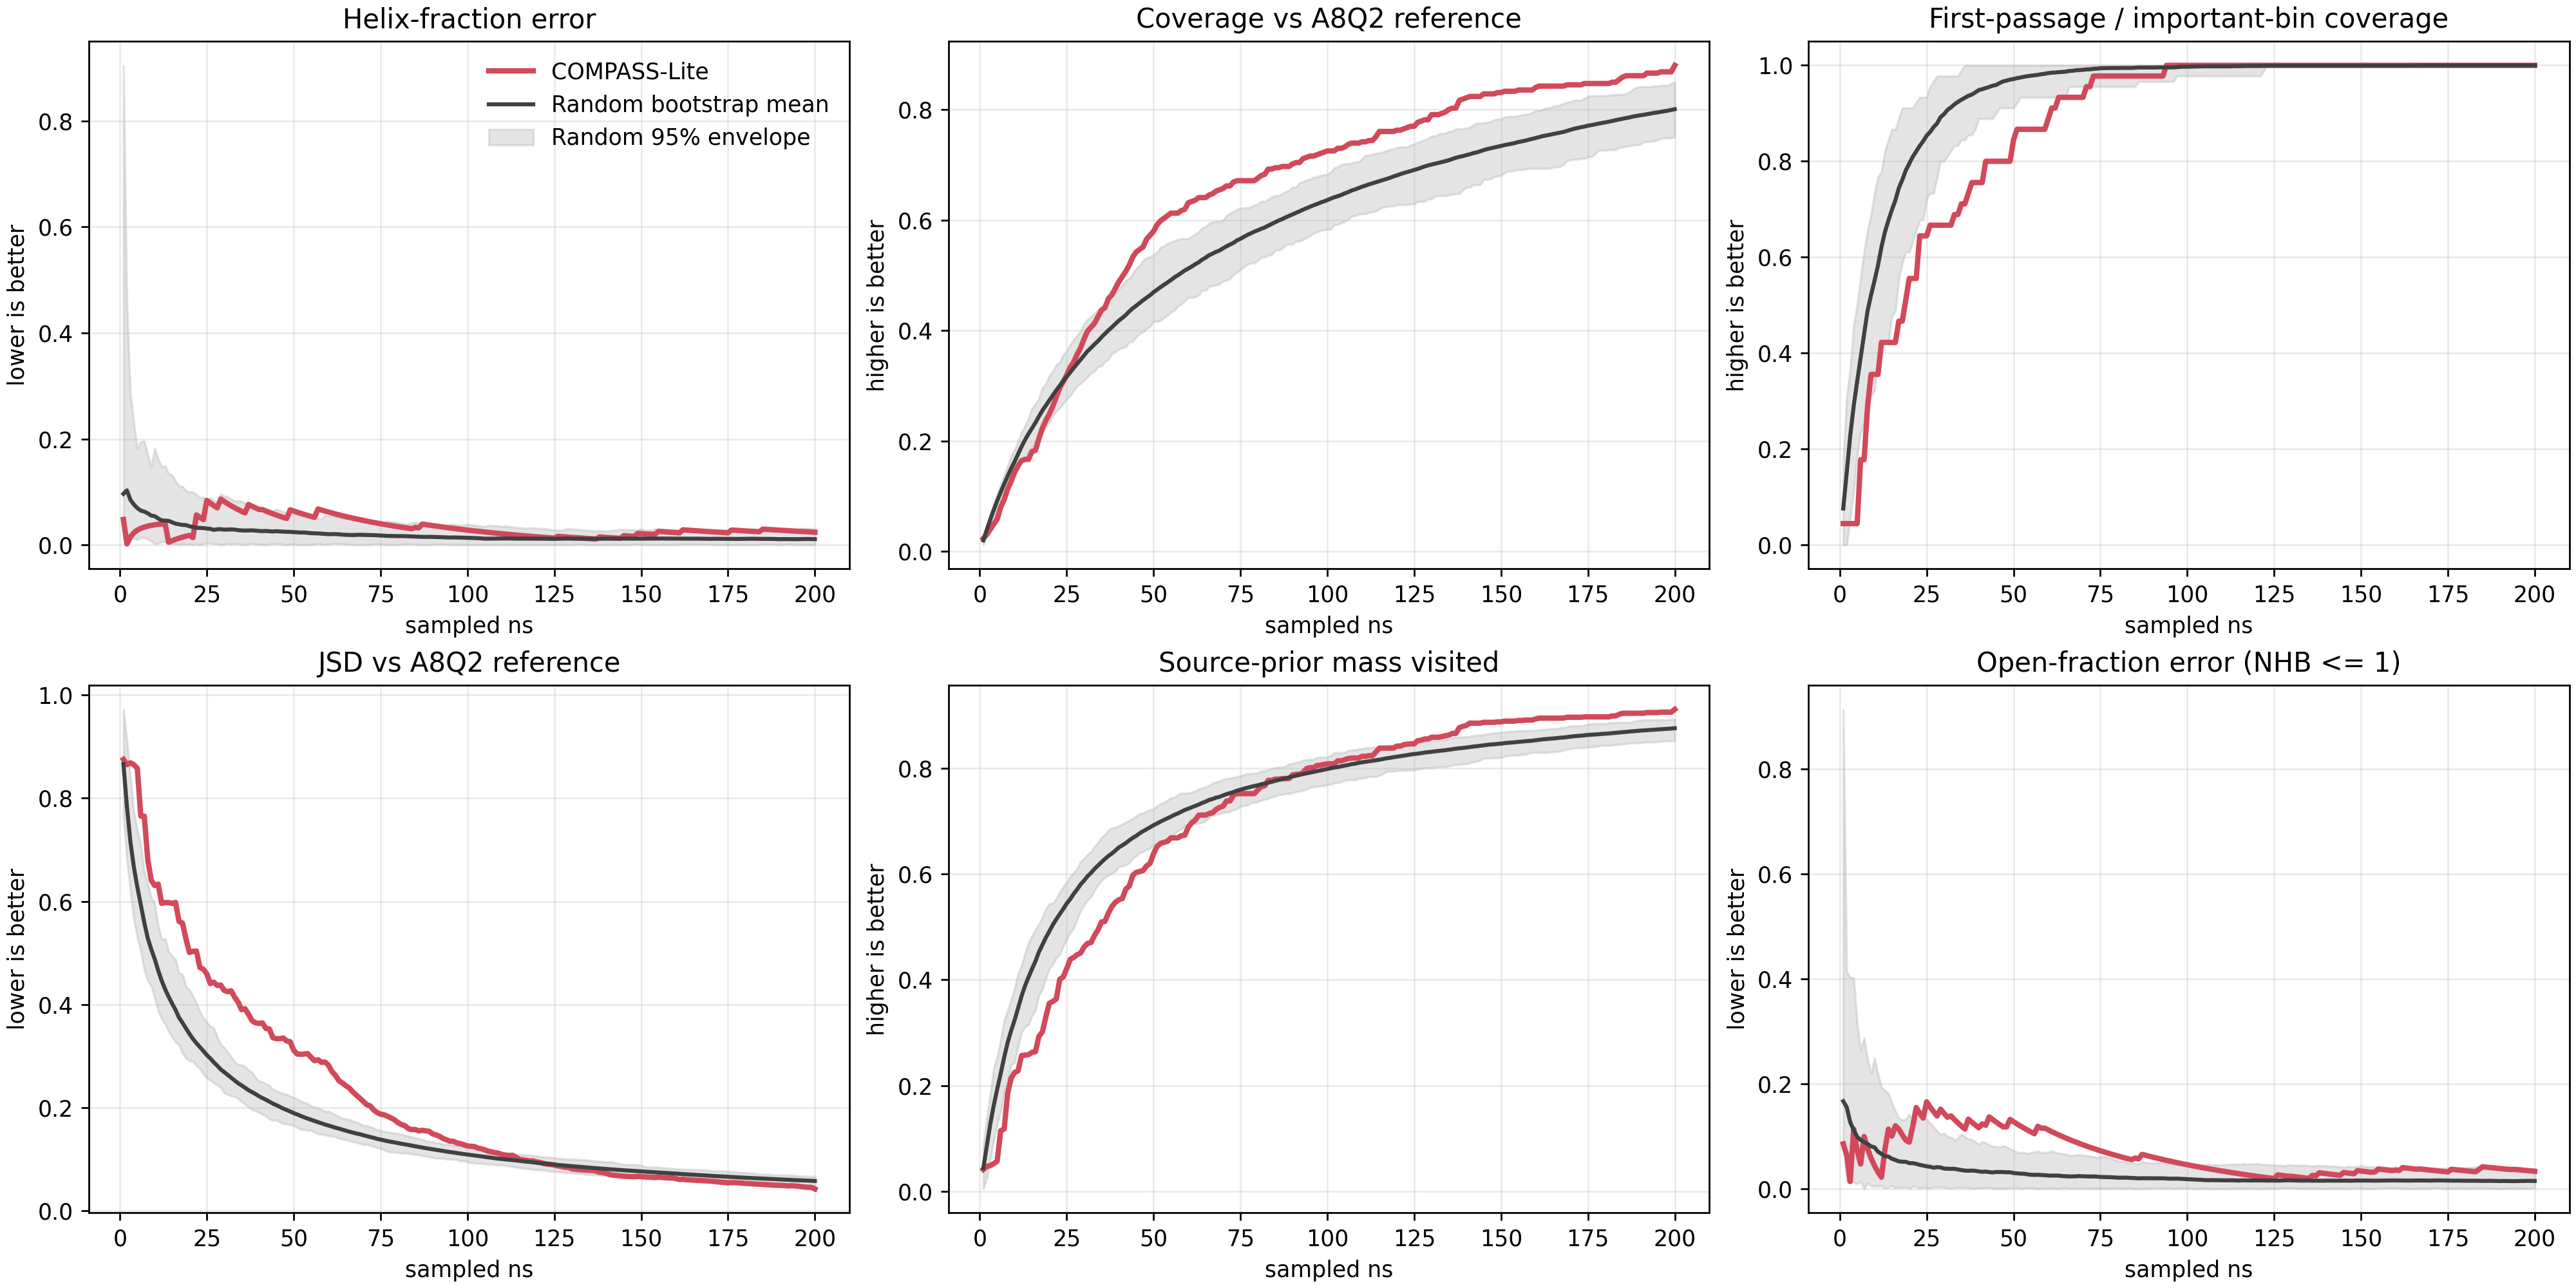
\includegraphics[width=0.92\linewidth]{replay_tica2d_200ns.png}
    \caption{Long-budget TICA2D acquisition ($200$\,ns total, $T_c=1$\,ns chunks). Same metric panels as Fig.~\ref{fig:tica80}. At $200$\,ns the TICA2D two-phase policy improves JSD, raw coverage, and source-mass visitation relative to bootstrap random acquisition, showing that the short-budget distributional penalty can be overcome with sufficient budget.}
    \label{fig:tica200}
\end{figure*}

\subsection{Prior Quality Controls the Failure Mode}
\label{sec:prior_quality}

Deliberately corrupted TICA priors showed that COMPASS follows its prior rather than ignoring it. A uniform prior increased coverage but degraded JSD and observables. A shuffled prior improved coverage and important coverage but no longer improved distributional accuracy. The inverted prior produced the strongest failure: JSD increased to 0.273 compared with 0.132 for random, and helix/open errors were substantially worse than random. A noisy prior was less damaging and remained closer to random.

\begin{table*}[htbp]
    \centering
    \caption{Selected $80$\,ns prior-quality tests for TICA2D two-phase acquisition ($T_c=1$\,ns chunks). \emph{Clean} denotes the uncorrupted A10 prior (\texttt{prior\_quality\,=\,none} in the code). Lower JSD and lower observable errors are better.}
    \label{tab:prior_quality}
    \begin{tabular}{lcccccc}
        \toprule
        Prior & JSD & Random JSD & Coverage & Random coverage & Helix error & Open error \\
        \midrule
        Clean & 0.147 & 0.132 & 0.528 & 0.583 & 0.0045 & 0.0066 \\
        Uniform & 0.200 & 0.132 & 0.765 & 0.583 & 0.0695 & 0.1079 \\
        Shuffled & 0.151 & 0.132 & 0.725 & 0.583 & 0.0208 & 0.0716 \\
        Inverted & 0.273 & 0.132 & 0.725 & 0.583 & 0.0645 & 0.1154 \\
        Noisy & 0.140 & 0.132 & 0.563 & 0.583 & 0.0245 & 0.0216 \\
        \bottomrule
    \end{tabular}
\end{table*}

The inverted-prior result is mechanistically useful even though it is a performance failure. It proves that the source prior is active in the policy. It also shows that prior trust cannot be treated as a minor implementation detail: a bad prior can actively steer acquisition toward the wrong target distribution.

\begin{figure*}[htbp]
    \centering
    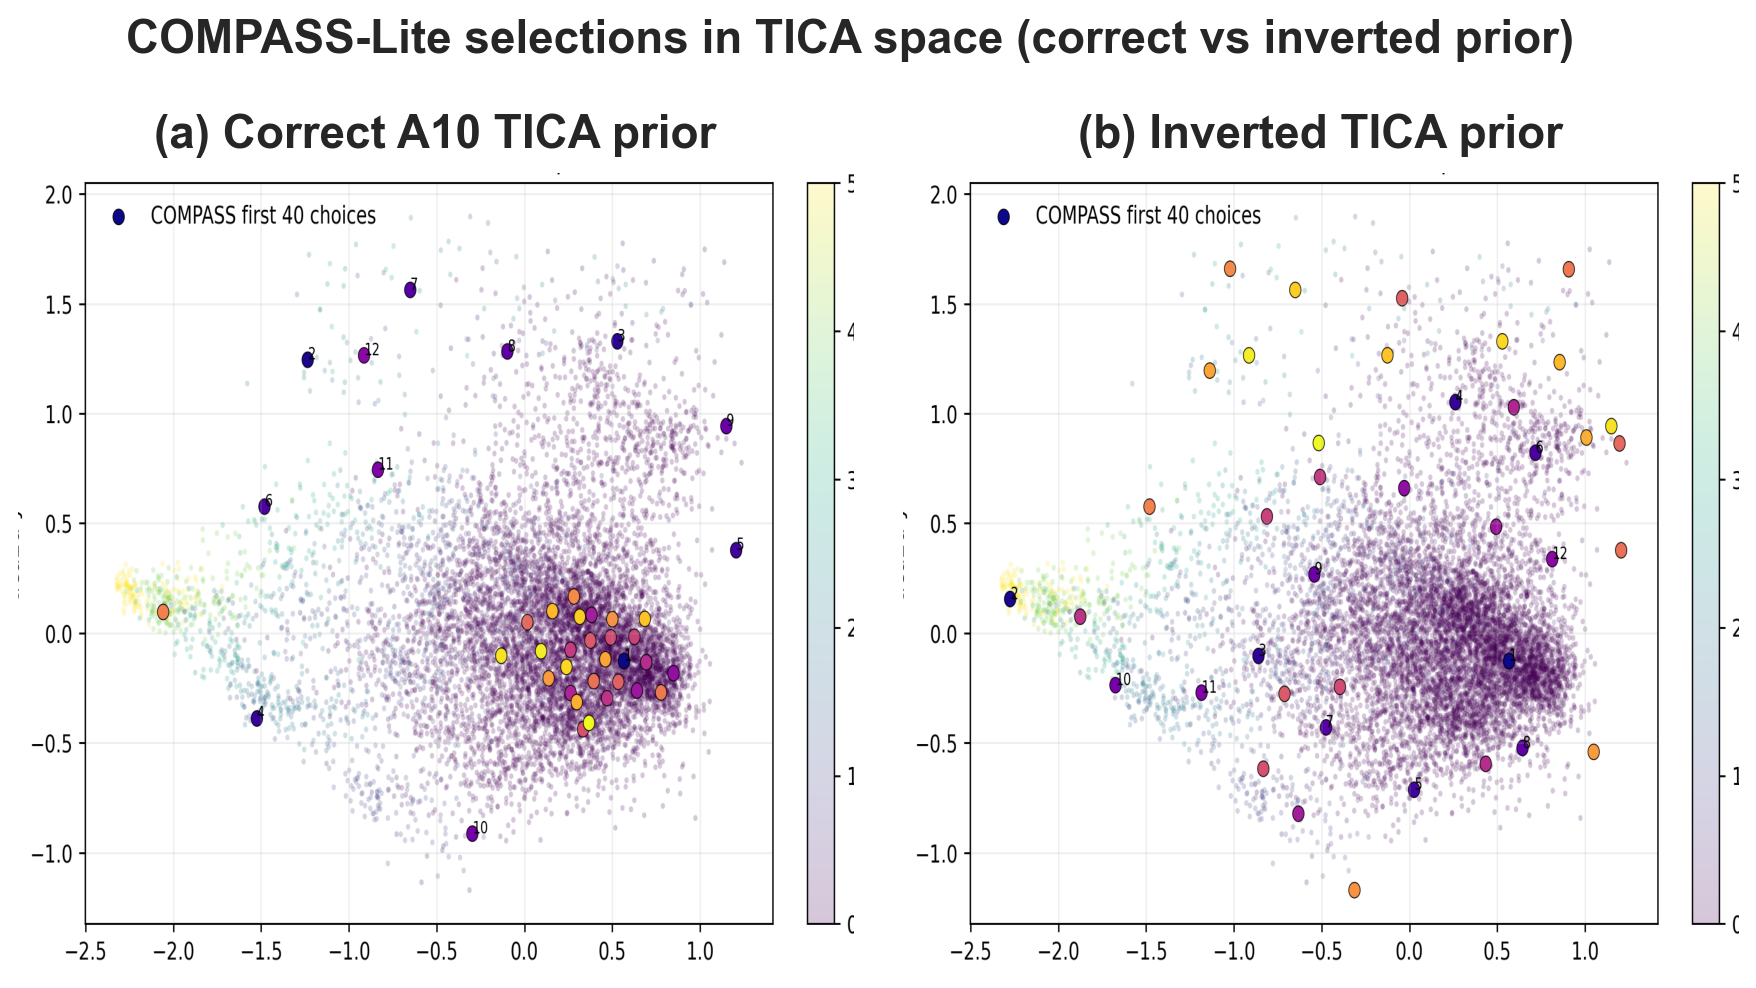
\includegraphics[width=0.92\linewidth]{prior_corruption_probe_maps.png}
    \caption{COMPASS chunk selections in TICA space under (a)~the correct A10 TICA prior and (b)~the inverted TICA prior. Background points show the A8Q2 target trajectory colored by hydrogen-bond count (yellow = high helix, purple = open); large numbered circles mark the first 40 COMPASS selections. Under the correct prior, selections concentrate in the dense core where most source-supported mass lies. Under the inverted prior, selections scatter into the sparse periphery, visually confirming that the policy follows its prior and that an inverted prior actively steers selection away from the target distribution.}
    \label{fig:prior_maps}
\end{figure*}

\subsection{Matched-Dynamics Benchmark Isolates Prior and Adaptivity Contributions}
\label{sec:results_msm}

On the MSM emulator described in Section~\ref{sec:methods_msm}, COMPASS (B6) is either the best or statistically tied (within one standard deviation) with the best policy on the helix- and open-fraction errors in every preset, and is the lowest-JSD policy in four of five presets (the sole exception being SPIB1D, where B0's fast 1D Markov mixing wins; see below), across 50 repeats (Table~\ref{tab:msm_benchmark}, Figs.~\ref{fig:msm_grid}--\ref{fig:msm_map}). The ordering against the other \emph{adaptive} baselines --- independent replicas (B1), uniform (B2), count-based min-count (B3), farthest-point (B4) --- is stable across presets and physically interpretable.

The long-budget tICA2D preset is the cleanest case. At 400\,ns of sampled time, COMPASS reduces the final-budget helix-fraction error to $\epsilon_{\mathrm{helix}}=1.9\times10^{-2}$, compared with $3.6\times10^{-2}$ for count-based min-count (B3) and $4.5\times10^{-2}$ for independent replicas (B1); the open-fraction error drops to $3.1\times10^{-2}$ versus $1.06\times10^{-1}$ for B3 and $8.1\times10^{-2}$ for B1. In the same preset COMPASS also edges out the single-walk diagnostic ceiling B0 on JSD ($0.316$ vs.\ $0.334$) and on both observables ($0.019$ vs.\ $0.024$; $0.031$ vs.\ $0.039$), despite B0 paying zero restart cost under Markov dynamics. On the $160$\,ns tICA2D baseline preset, COMPASS is already the best JSD policy ($0.509$ vs.\ $0.524$ for B0) and the best helix-error policy ($0.028$), while open error ($0.045$) differs negligibly from B2 uniform ($0.043$) at the level of repeat-to-repeat scatter.

Three policy-level observations survive the preset-averaged view. First, \emph{the prior contribution} $B6{-}B3$ is \emph{strictly} negative on mean final JSD in all five presets (largest gaps on SPIB1D, $\approx -0.14$, and long-budget tICA2D, $\approx -0.06$), and is negative on mean $\epsilon_{\mathrm{helix}}$ in three of five presets (on the tICA baseline and two-seed presets the helix mean difference is positive but within repeat noise); see Fig.~\ref{fig:msm_pair}, top two rows. Second, \emph{the adaptivity contribution} $B3{-}B1$ is negative on JSD in every preset, and negative on $\epsilon_{\mathrm{helix}}$ in four of five presets --- the lone exception is SPIB1D, where min-count's aggressive targeting of under-sampled bins on the coarse 1D grid over-represents the minority (helix) state and produces a \emph{worse} helix error than plain replicas. This pathology of pure count-based targeting is itself instructive and is discussed alongside the SPIB1D caveats in the next paragraph. Third, and mechanistically the most pointed result, farthest-point exploration (B4) \emph{catastrophically} biases equilibrium observables on the tICA presets: $|\Delta f_{\mathrm{open}}|$ for B4 reaches $0.33$--$0.48$ because pure-geometric ``novelty'' drives restarts into peripheral bins that carry essentially no equilibrium mass, so the cumulative histogram under-represents the helical core. Bin coverage for B4 sits at the bottom of the policy ranking on the tICA presets ($0.06$--$0.20$, comparable to non-adaptive replicas), so this is not a coverage-for-observables trade-off: geometric exploration is simply wasting budget on bins with vanishing occupancy. Figure~\ref{fig:msm_map} makes the spatial pattern explicit on the long-budget tICA preset: mean sampled mass for B4 is pushed into peripheral bins (red in the $\ln(\mathrm{sample}/\mathrm{ref})$ panels) while COMPASS (B6) stays closer to the equilibrium core. This is the matched-dynamics echo of the inverted-prior failure in Section~\ref{sec:prior_quality}: ``more exploration'' is not automatically useful; what matters is whether exploration respects the source density or a validated proxy for it.

Two results are deliberately presented with caution. On the SPIB1D preset, B0's very low final JSD ($6.3\times10^{-2}$) reflects the 1D discretization's fast Markov mixing on that grid rather than any property of ``running one long trajectory'' --- B0 is an emulator-level ceiling, not a real-MD competitor, and pricing restarts at zero is what gives it the narrow JSD lead. And on the same preset, count-based B3 (and the purely geometric B4, which is slightly worse still) inflate both observables by an order of magnitude over COMPASS ($|\Delta f_{\mathrm{helix}}|=0.21$, $|\Delta f_{\mathrm{open}}|=0.26$ for B3 vs.\ $0.037$, $0.045$ for B6): without a density prior, pure under-sampled-state targeting over-represents minority-state bins on a 1D grid. Both observations reinforce, rather than weaken, the central claim that the prior is doing identifiable work.

\begin{table*}[htbp]
    \centering
    \caption{MSM-emulator benchmark: final-budget means across 50 repeats for three representative presets. Lower is better for JSD, $|\Delta f_{\mathrm{helix}}|$, $|\Delta f_{\mathrm{open}}|$; higher is better for coverage. Best entry in each column is \textbf{bold}. B0 is the single-walk diagnostic ceiling under Markov dynamics and is optimistic relative to real MD restart cost. Full five-preset table is in the Supporting Information.}
    \label{tab:msm_benchmark}
    \small
    \setlength{\tabcolsep}{4pt}
    \begin{tabular}{llcccc}
        \toprule
        Preset & Policy & JSD $\downarrow$ & Coverage $\uparrow$ & $|\Delta f_{\mathrm{helix}}|$ $\downarrow$ & $|\Delta f_{\mathrm{open}}|$ $\downarrow$ \\
        \midrule
        \multirow{6}{*}{tICA2D baseline, 160\,ns} & B0 single-walk & 0.524 & 0.142 & 0.038 & 0.067 \\
        & B1 replicas & 0.618 & 0.106 & 0.044 & 0.080 \\
        & B2 uniform & 0.521 & 0.137 & 0.037 & \textbf{0.043} \\
        & B3 min-count & 0.534 & 0.142 & 0.038 & 0.067 \\
        & B4 farthest & 0.735 & 0.102 & 0.090 & 0.381 \\
        & B6 COMPASS & \textbf{0.509} & 0.142 & \textbf{0.028} & 0.045 \\
        \midrule
        \multirow{6}{*}{SPIB1D, 160\,ns} & B0 single-walk & \textbf{0.063} & 0.540 & \textbf{0.025} & \textbf{0.031} \\
        & B1 replicas & 0.320 & 0.599 & 0.053 & 0.088 \\
        & B2 uniform & 0.117 & 0.625 & 0.084 & 0.106 \\
        & B3 min-count & 0.213 & \textbf{0.756} & 0.215 & 0.264 \\
        & B4 farthest & 0.319 & 0.725 & 0.247 & 0.286 \\
        & B6 COMPASS & 0.077 & 0.545 & 0.037 & 0.045 \\
        \midrule
        \multirow{6}{*}{tICA2D long, 400\,ns} & B0 single-walk & 0.334 & 0.285 & 0.024 & 0.039 \\
        & B1 replicas & 0.555 & 0.156 & 0.045 & 0.081 \\
        & B2 uniform & 0.359 & 0.270 & 0.031 & 0.034 \\
        & B3 min-count & 0.374 & \textbf{0.290} & 0.036 & 0.106 \\
        & B4 farthest & 0.646 & 0.202 & 0.040 & 0.479 \\
        & B6 COMPASS & \textbf{0.316} & 0.277 & \textbf{0.019} & \textbf{0.031} \\
        \bottomrule
    \end{tabular}
\end{table*}

\begin{figure*}[htbp]
    \centering
    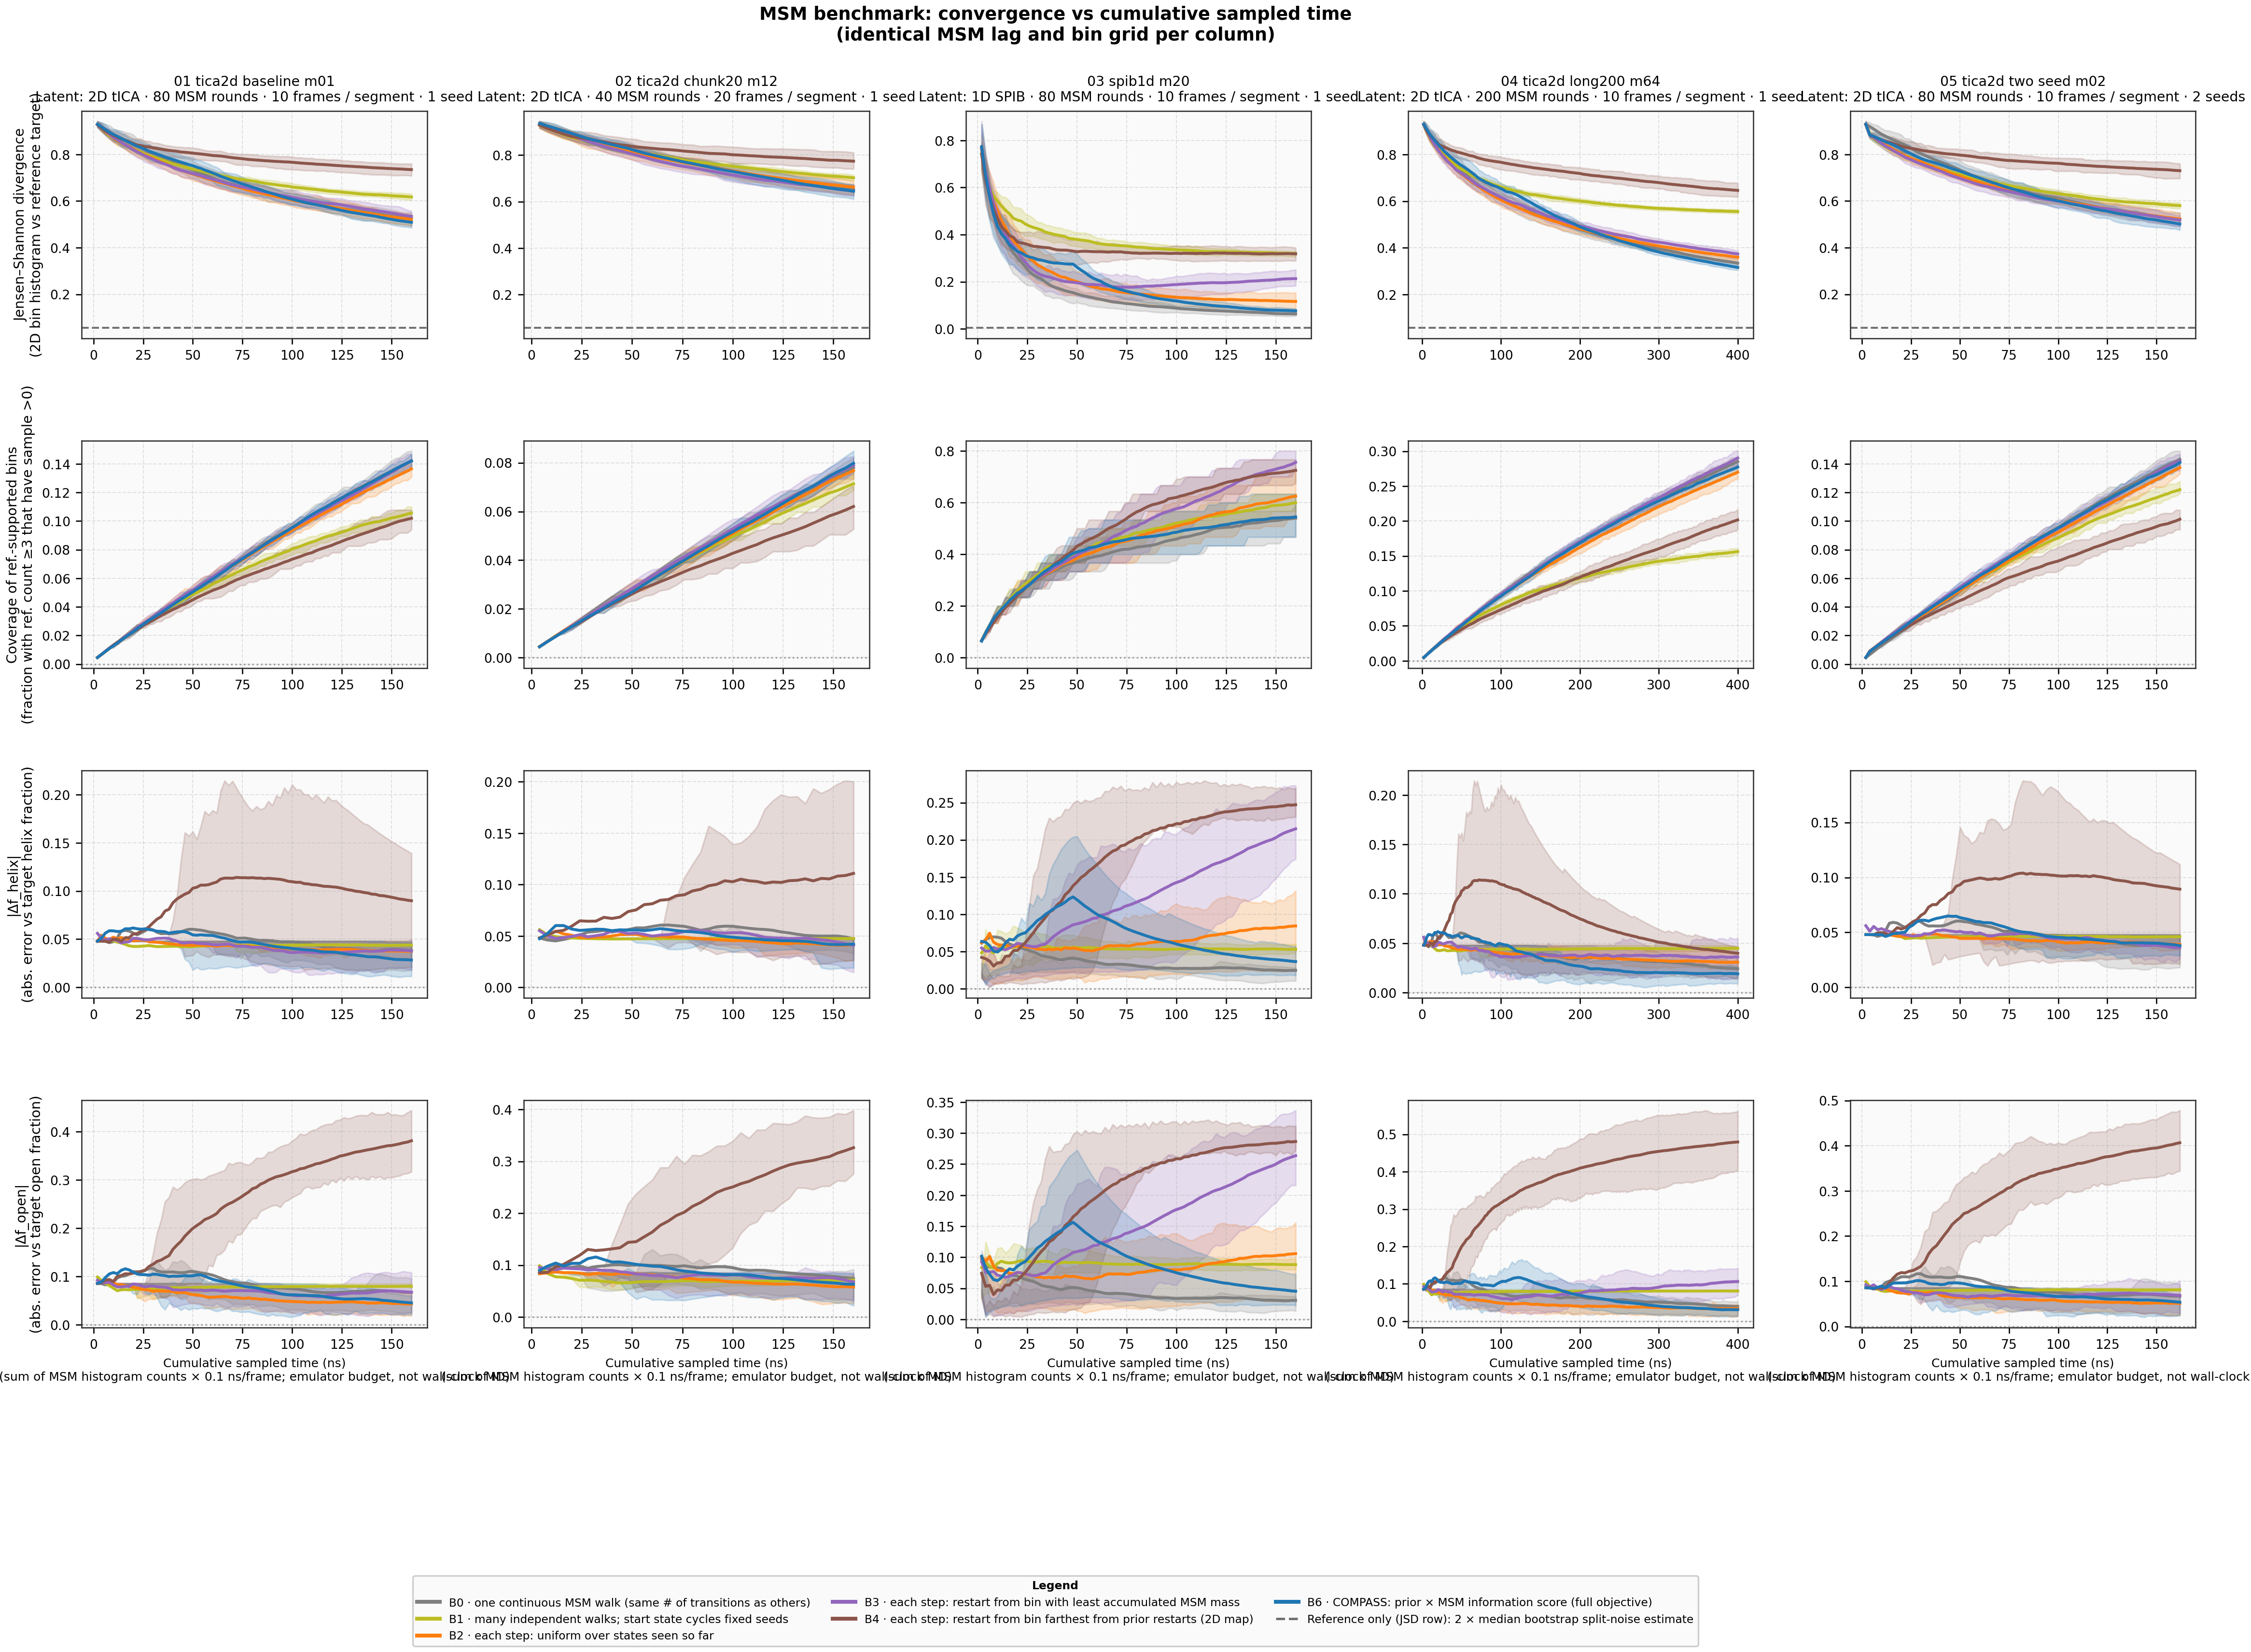
\includegraphics[width=0.95\linewidth]{msm_convergence_grid.png}
    \caption{MSM-emulator benchmark: convergence of four metrics (rows: JSD, coverage of reference-supported bins, $|\Delta f_{\mathrm{helix}}|$, $|\Delta f_{\mathrm{open}}|$) versus lag-weighted cumulative sampled time (ns), across five preset configurations (columns). Lines show means; shaded bands show the interquartile range across 50 independent repeats. Horizontal dashed line on the JSD row is twice the median bootstrap split-noise estimate for that preset. Across every preset, COMPASS (B6, blue) matches or beats count-based min-count (B3, purple) and independent replicas (B1, olive) on the two observable errors, while farthest-point exploration (B4, brown) diverges on $|\Delta f_{\mathrm{open}}|$ in all tICA presets.}
    \label{fig:msm_grid}
\end{figure*}

\begin{figure*}[htbp]
    \centering
    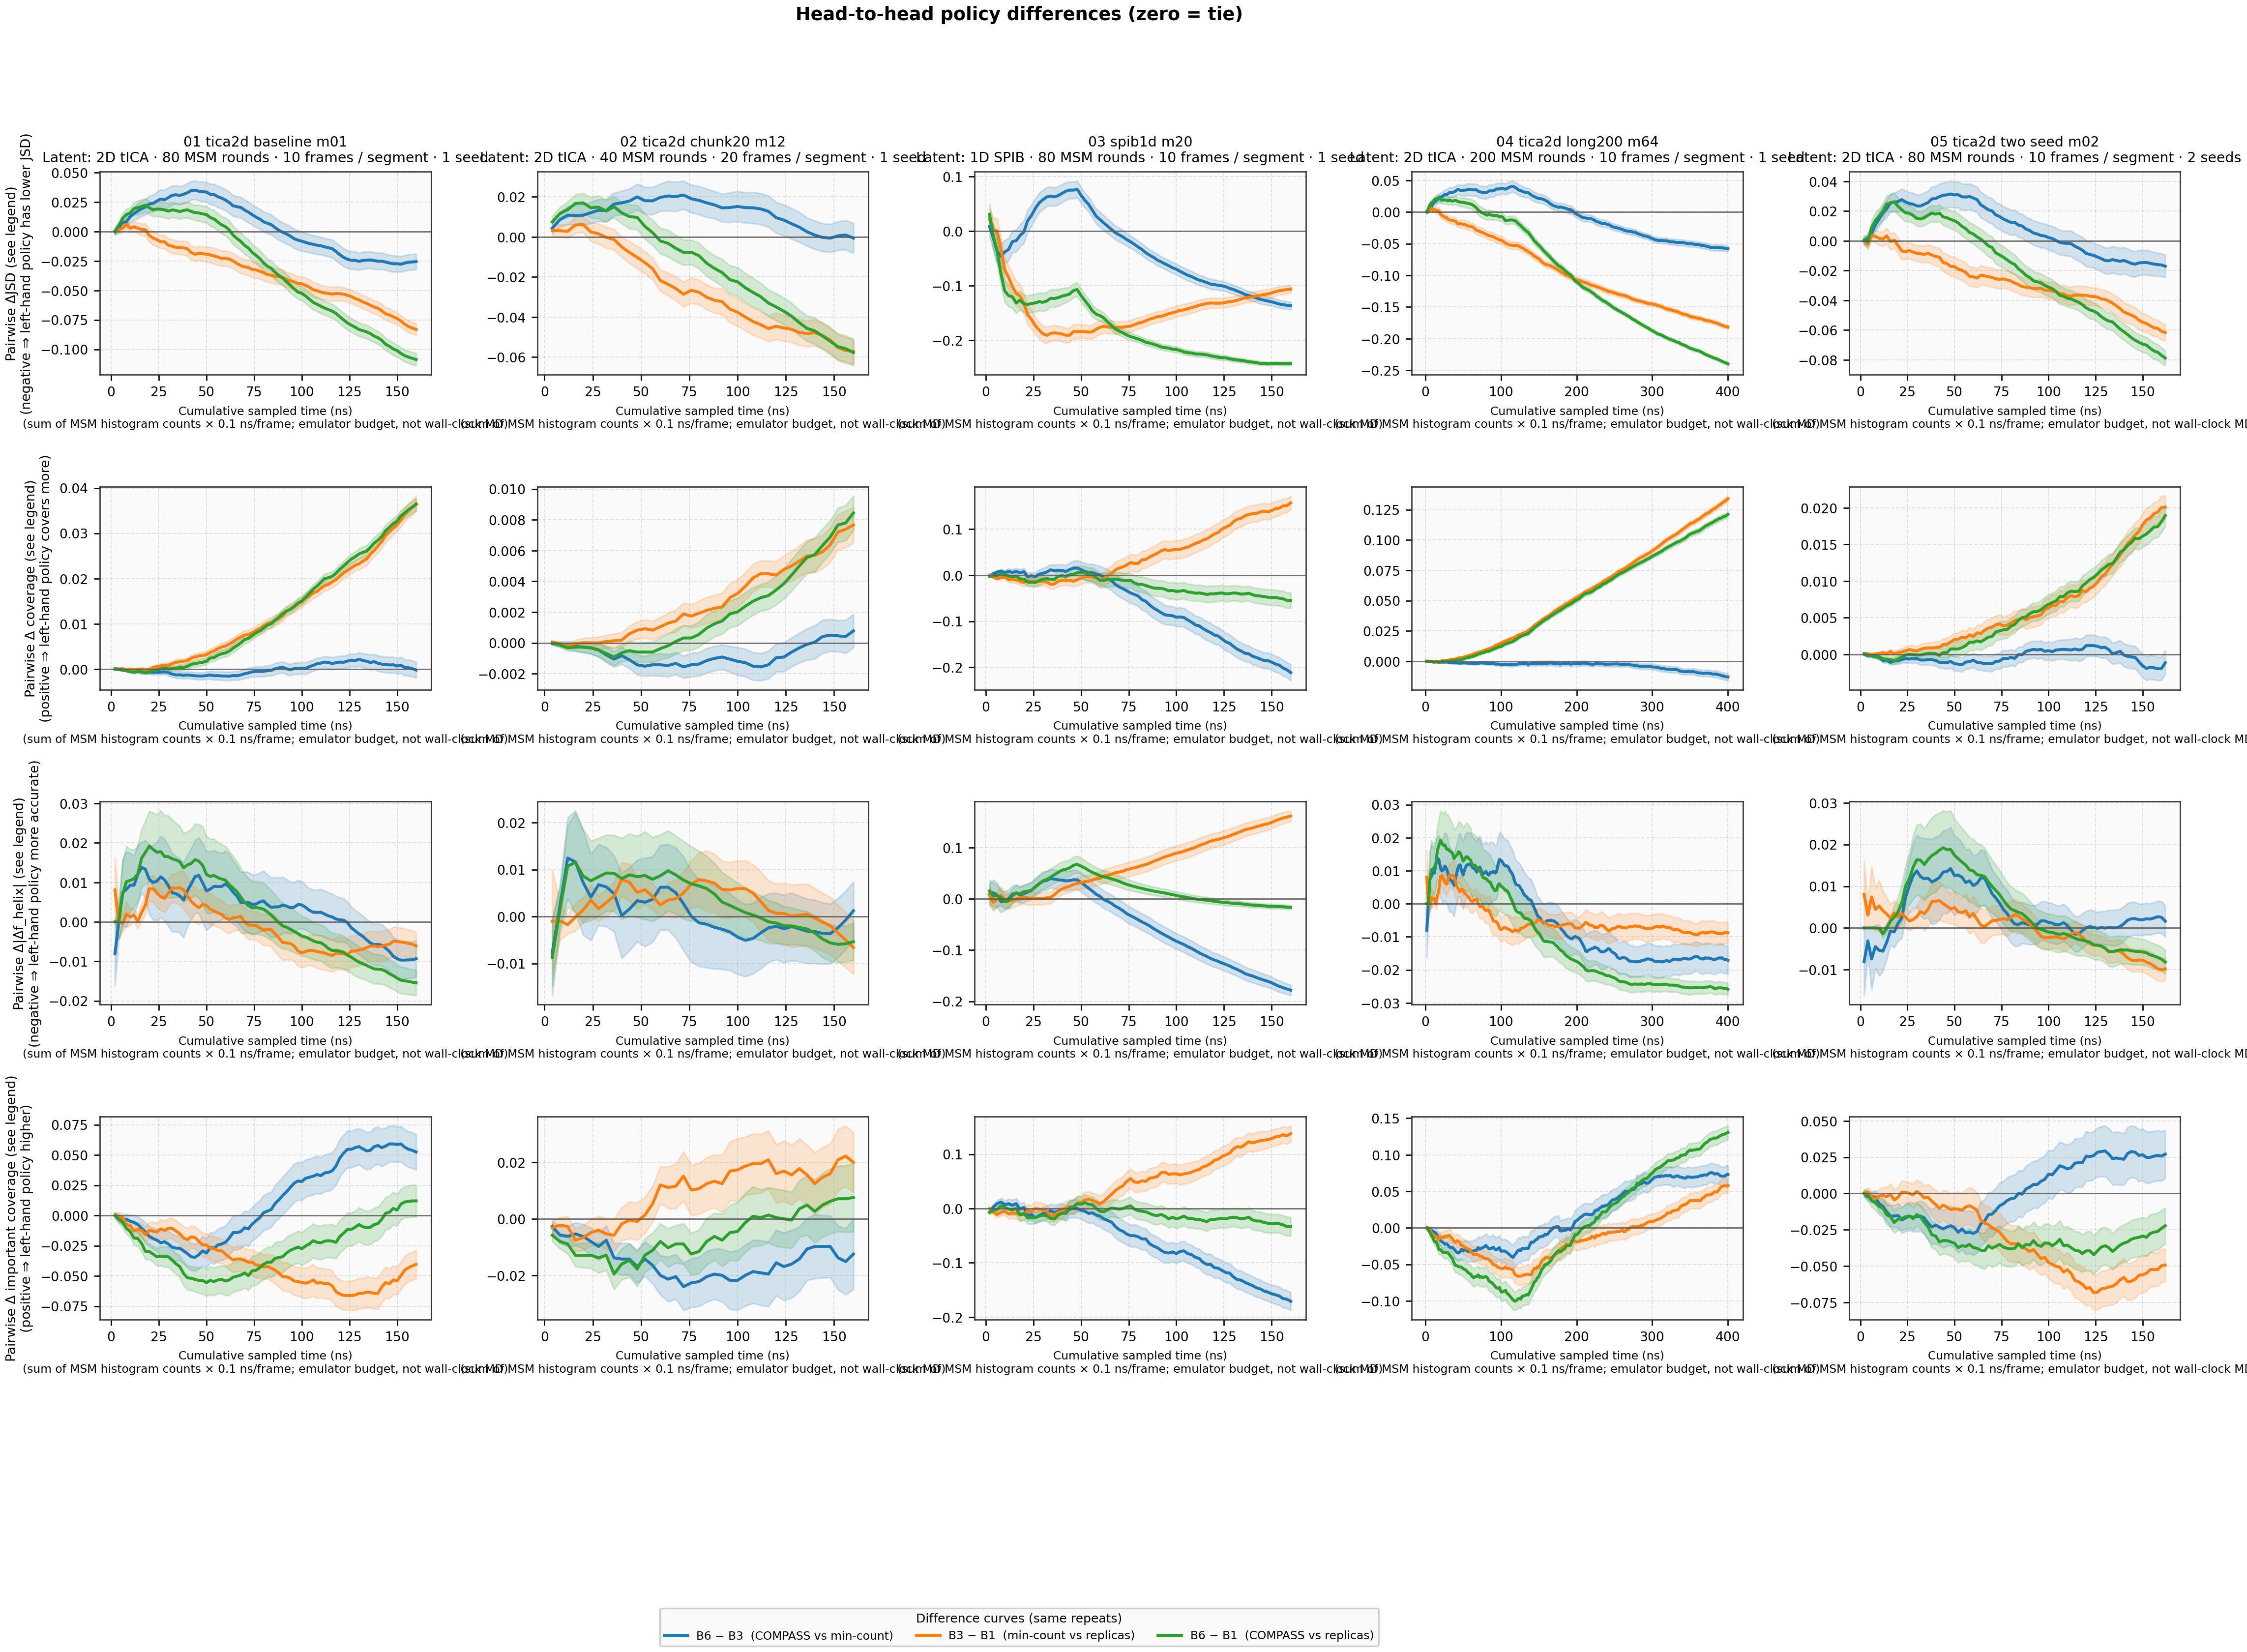
\includegraphics[width=0.95\linewidth]{msm_pair_delta_curves.png}
    \caption{Head-to-head pair differences along the same random repeats of Fig.~\ref{fig:msm_grid}: $B6-B3$ (COMPASS minus min-count, isolating the \emph{prior contribution}), $B3-B1$ (min-count minus replicas, isolating the \emph{adaptivity contribution}), and $B6-B1$ (total lift). For JSD and $|\Delta f_{\mathrm{helix}}|$ a negative value favors the first-named policy; for coverage-like metrics the sign flips (see panel titles). Mean $B6-B3$ on JSD is negative in every preset. The two contributions compound on average: COMPASS tracks the reference more closely than either count-based adaptive sampling alone or non-adaptive replicas alone.}
    \label{fig:msm_pair}
\end{figure*}

\begin{figure*}[htbp]
    \centering
    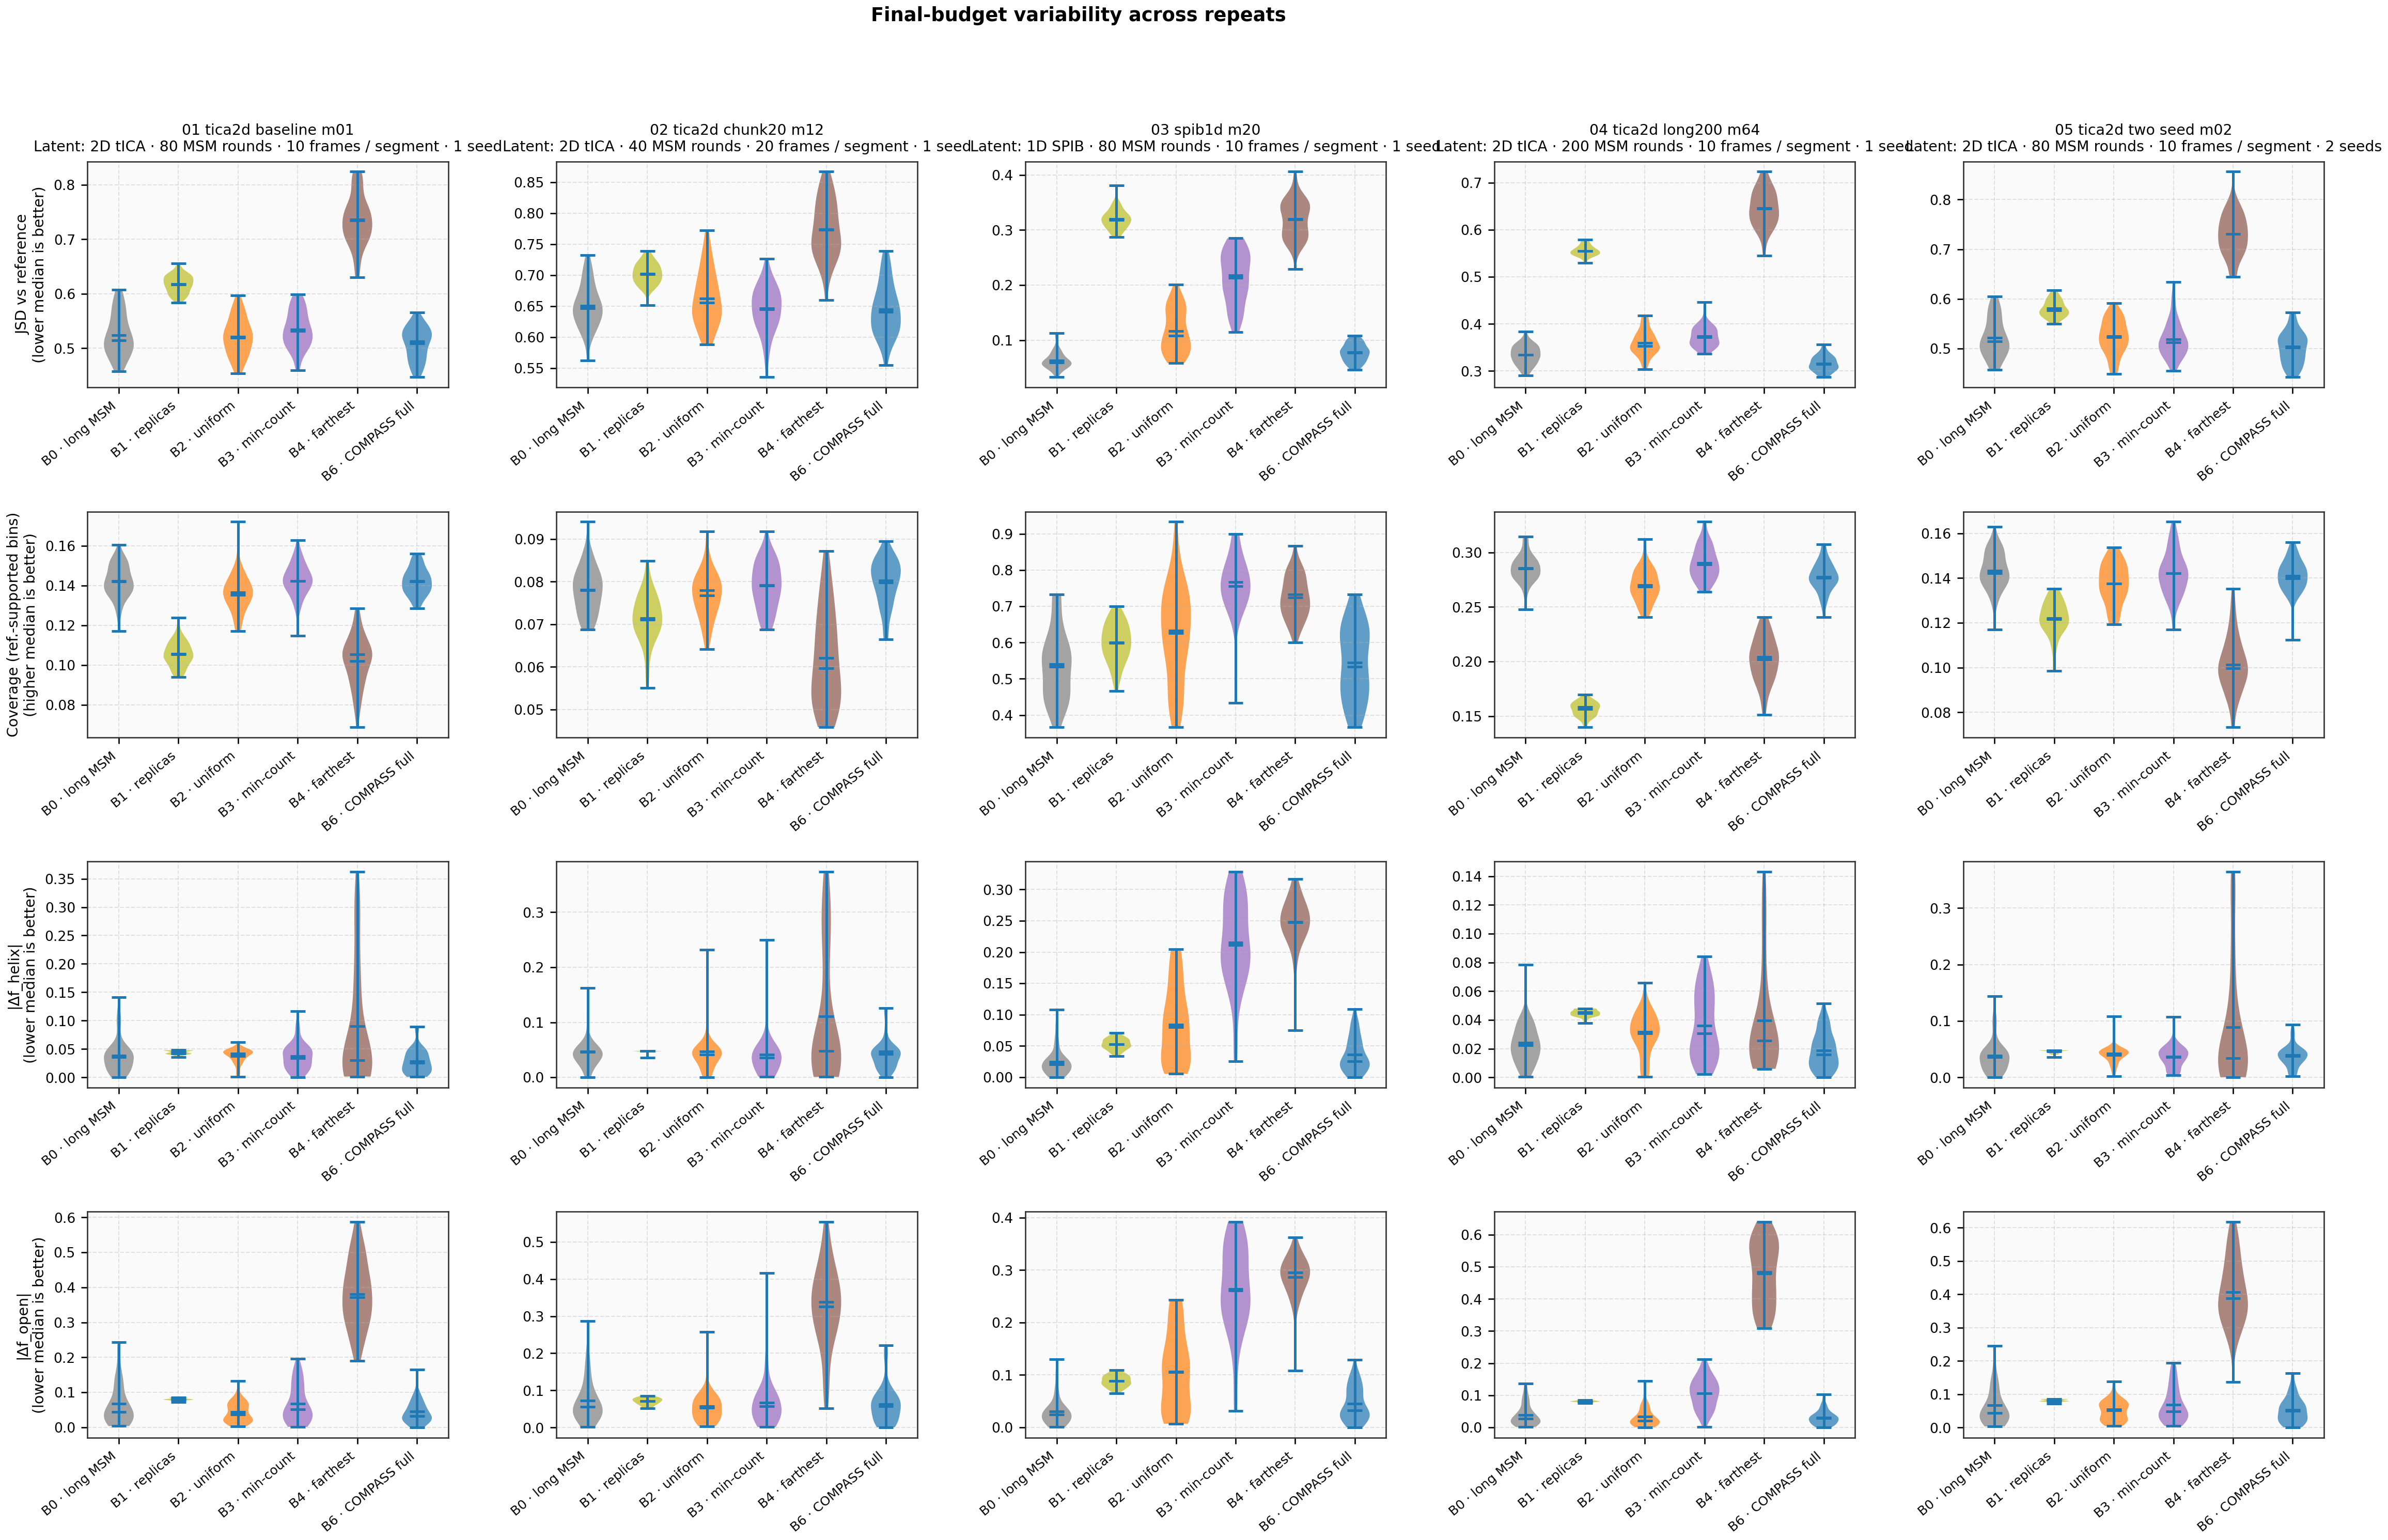
\includegraphics[width=0.95\linewidth]{msm_final_budget_violins.png}
    \caption{MSM-emulator benchmark: full repeat-level variability at the \emph{final} simulated round (violins; one draw per repeat per policy), for the same five presets and policies as Fig.~\ref{fig:msm_grid}. Rows are JSD, reference-supported coverage, $|\Delta f_{\mathrm{helix}}|$, and $|\Delta f_{\mathrm{open}}|$; violins are ordered by policy along the horizontal axis within each preset column. This view complements mean trajectories and pair-difference curves: it highlights multi-modal or heavy-tailed failure modes---notably wide $|\Delta f_{\mathrm{helix}}|$ and $|\Delta f_{\mathrm{open}}|$ spreads for min-count (B3) and farthest-point (B4) on SPIB1D and the exploding $|\Delta f_{\mathrm{open}}|$ tails for B4 on the tICA presets.}
    \label{fig:msm_violins}
\end{figure*}

\begin{figure*}[htbp]
    \centering
    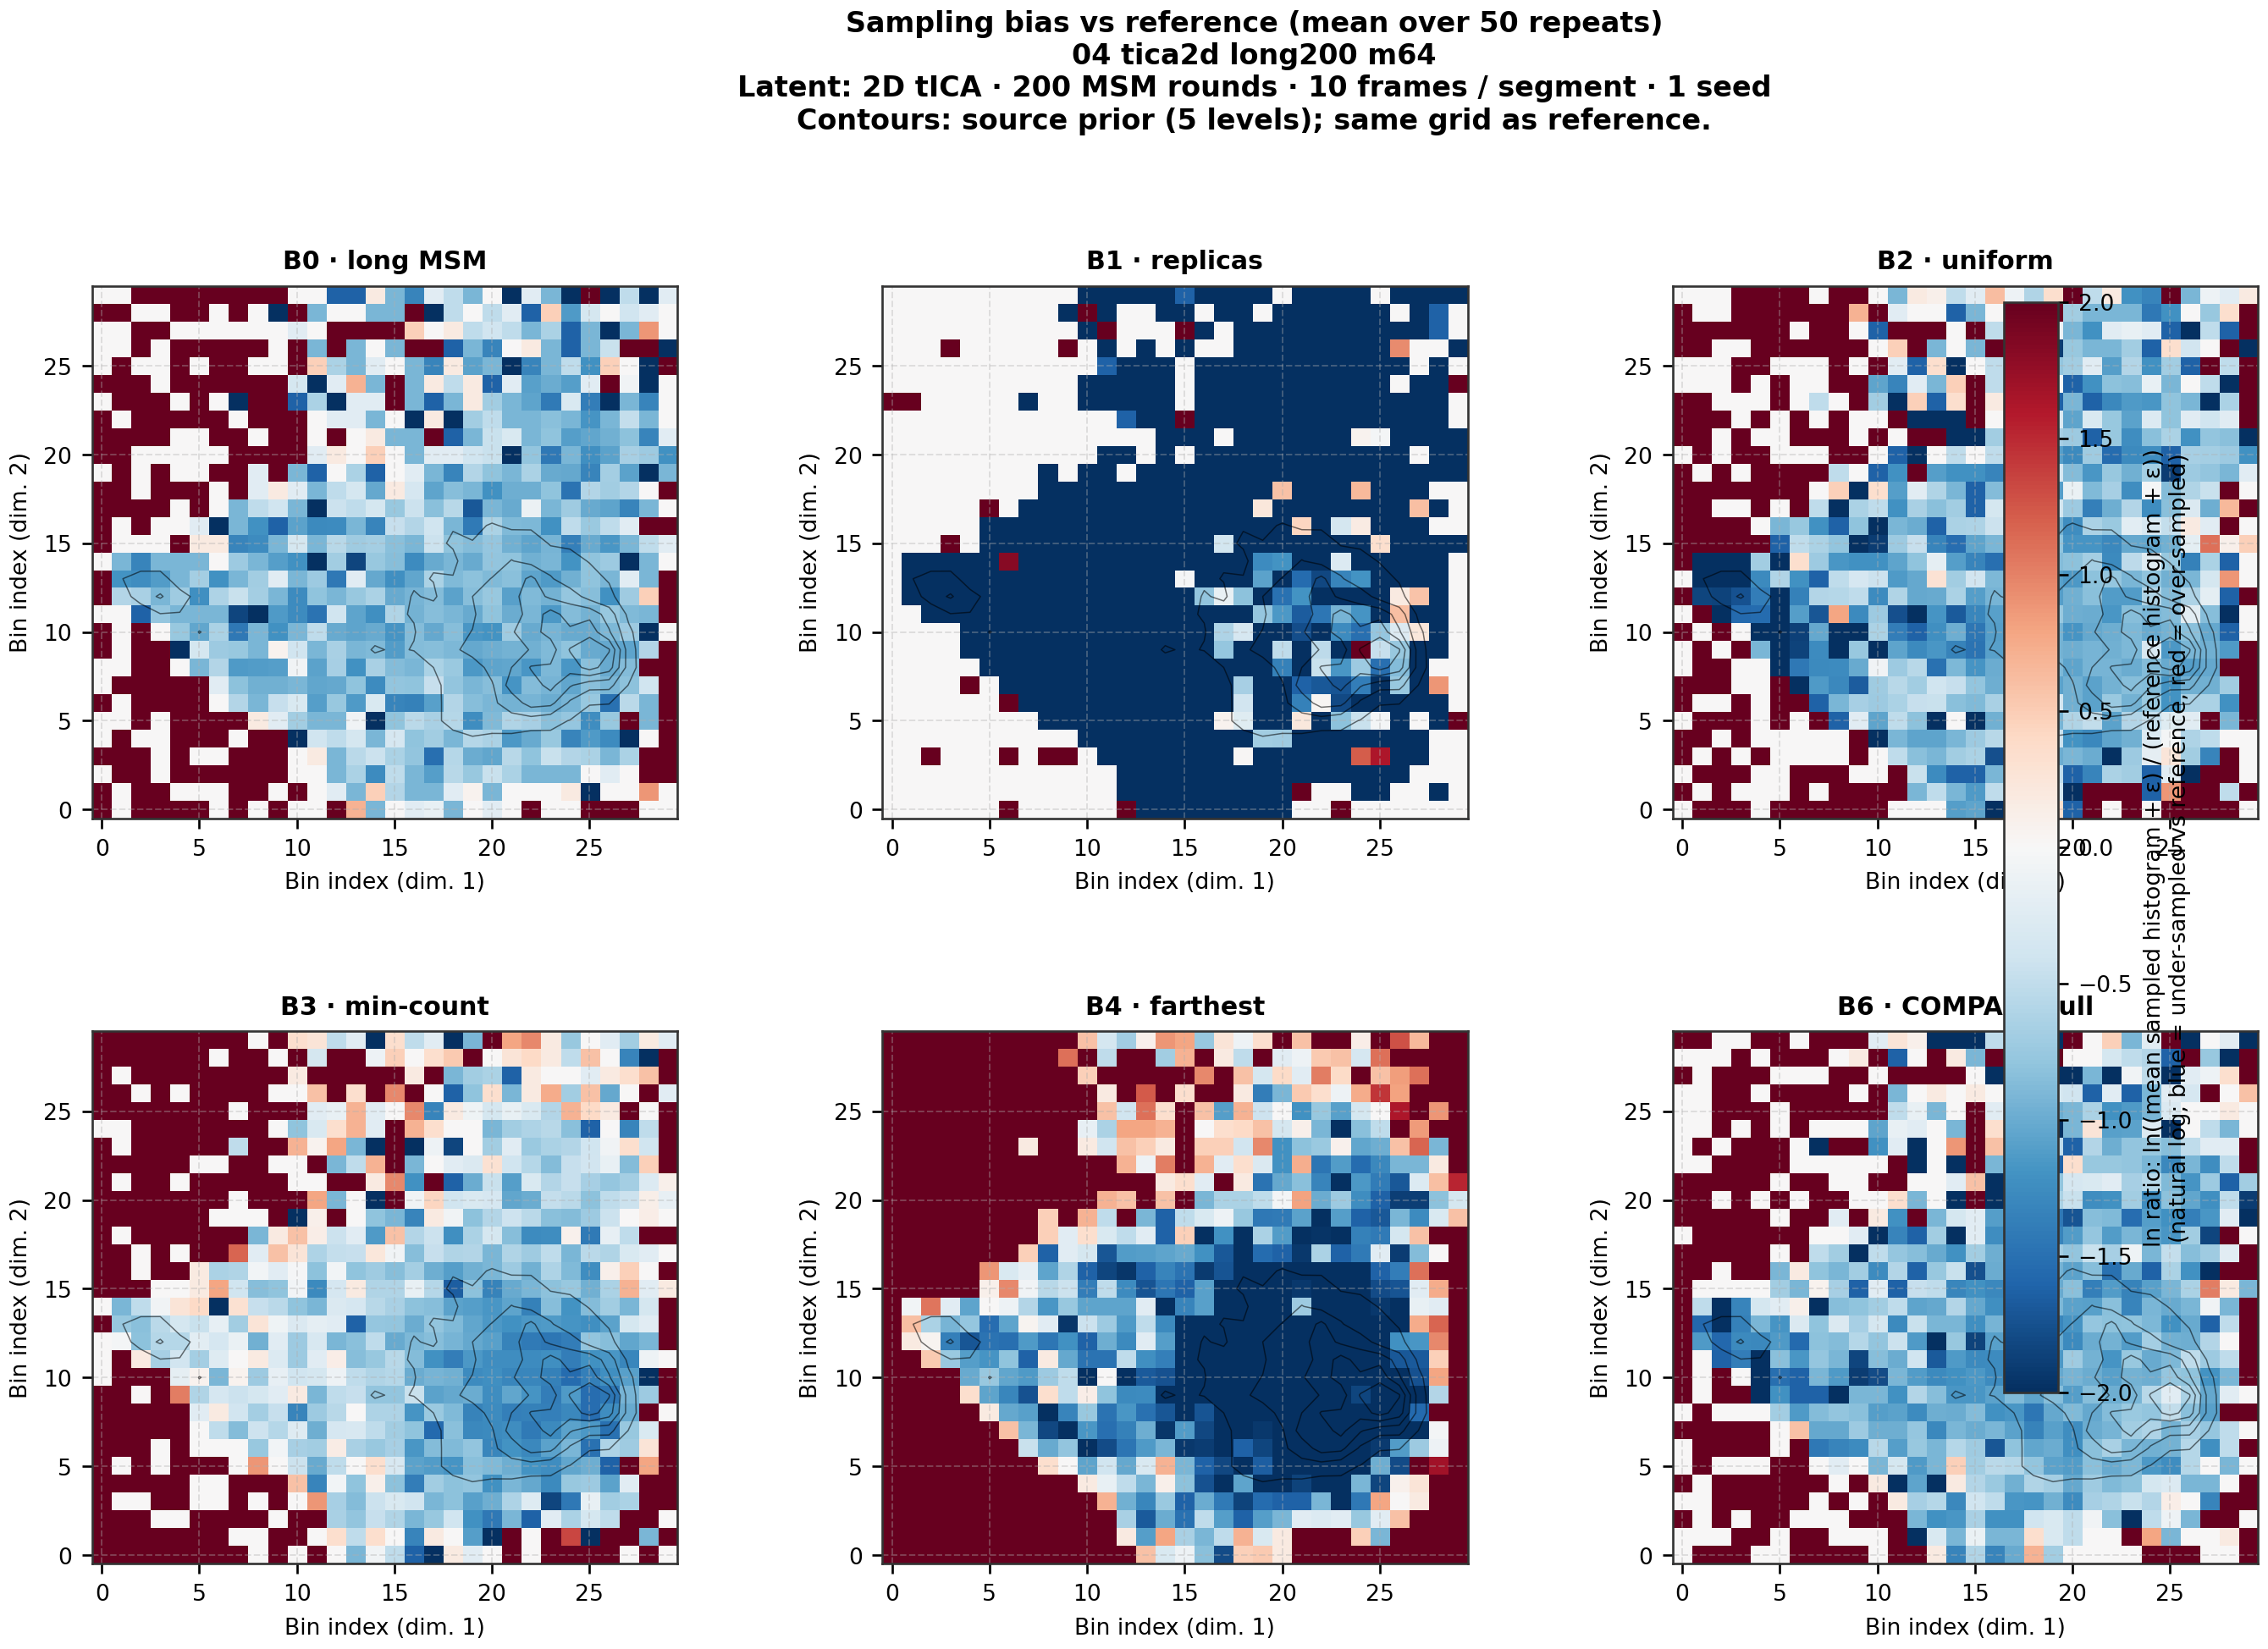
\includegraphics[width=0.95\linewidth]{msm_map_overlay_tica2d_long400ns.png}
    \caption{MSM-emulator spatial view for the long-budget 2D tICA preset (400\,ns sampled time; same bins and reference as Table~\ref{tab:msm_benchmark}, long row). Each panel averages the final lag-weighted histogram over 50 repeats for the labeled policy and displays $\ln[(\mathrm{mean\ sampled\ mass}+\varepsilon)/(\mathrm{reference\ mass}+\varepsilon)]$ per bin (red\,=\,over-sampled versus reference, blue\,=\,under-sampled); black contours trace the source prior on the grid. Farthest-point restarts (B4) concentrate error in the map periphery, whereas COMPASS-full (B6) keeps mass closer to the core populated in the target reference. \emph{Note:} panel banners in the raster image still read ``Fig.~4'' from the plotting script; the journal's figure number will differ.}
    \label{fig:msm_map}
\end{figure*}

\section{Discussion}

\subsection{A Coherent Interpretation}

The results support a nuanced view of prior-guided adaptive acquisition. TICA2D is best treated as a density and observable prior. It is not globally transferable from A10 to A8Q2, but it carries enough helix-relevant information to improve selected observables under short budget and distributional recovery under longer budget. SPIB1D is best treated as a discovery accelerator. It rapidly visits source-supported latent regions but does not preserve equilibrium helix/open populations in this transferred setting.

The most important methodological lesson is that adaptive policies should not be judged by a single metric. Coverage, JSD, first-passage discovery, and observable errors report different aspects of success. In this benchmark, policies that maximize coverage can worsen equilibrium-like accuracy, while policies that match density can initially lose coverage before improving JSD at longer budget.

\subsection{Implications for Adaptive MD}

Many adaptive sampling methods balance exploration of under-sampled regions with exploitation of known progress coordinates.\cite{shamsi2018reap,yang2024werl,leung2025dlwe} Linear slow-coordinate methods such as TICA provide interpretable kinetic projections, whereas nonlinear latent models such as SPIB can reveal state-predictive manifolds in complex molecular data.\cite{perezhernandez2013tica,wang2021spib} COMPASS differs from rigorous weighted ensemble approaches because it does not assign trajectory weights and does not produce unbiased kinetic estimates from the selected chunks. Its role is instead diagnostic: it tests whether a proposed prior would make useful acquisition decisions before expensive online simulations are launched.

This distinction matters for interpreting the results correctly. The present results do not show that COMPASS directly accelerates online A8Q2 MD. They show that transferred latent priors contain usable but metric-specific information, and that retrospective acquisition can reveal when those priors are helpful or harmful. The natural next step is an online or semi-online validation in which the same acquisition policy launches new OpenMM trajectories from selected structures.

\subsection{Why Random Is a Strong Baseline}

The random baseline samples from the completed A8Q2 chunk library. It is therefore a strong retrospective comparator because it has access to the same high-quality target pool, even though it does not use labels or priors. The pattern in our results --- random hard to beat for global distributional coverage, transferred priors specifically helpful for selected observables --- should be read in this light: COMPASS's job is not to dominate random on every metric, but to identify the metrics on which a transferred prior demonstrably contributes signal.

\subsection{Design Principle: Control Prior Trust}

The prior-corruption experiments make trust calibration the central design principle. If the prior is good enough and the objective is density or helix-population recovery, TICA guidance can help. If the prior is bad, the policy follows it into failure. If the prior is replaced by an exploration-only objective (uniform row, Table~\ref{tab:prior_quality}), coverage improves at the cost of JSD and observables. Combining a discovery latent and a density latent without an explicit trust mechanism therefore raises a clear risk of objective interference, motivating a controlled-hybrid extension in future online work.

A future controller should estimate whether the density prior is currently paying off. SPIB frontier pressure could be activated only when important-bin discovery is incomplete or when TICA-density progress has stalled, and reduced once sufficient discovery has occurred so that density correction can dominate.

\subsection{Prior Value Survives Matched Dynamics}
\label{sec:disc_msm}

Section~\ref{sec:results_msm} already gives the quantitative MSM comparison; we highlight here only what it adds to the retrospective story. Under shared $\mathbf{T}$, lag, bins, seeds, and transition budget, the pair-difference view ($B6{-}B3$ vs.\ $B3{-}B1$) supports the same architectural reading as the scoring decomposition: prior-aware density steering and generic adaptivity are separable contributors, and neither alone explains the full COMPASS lift.

Two failure geometries rhyme with Section~\ref{sec:prior_quality} but are not identical. Retrospective inverted priors can raise bin coverage while worsening JSD and observables. On tICA MSM presets, farthest-point restarts instead steer mass to geometrically extreme, low-occupancy bins: coverage for B4 is among the lowest policies while $|\Delta f_{\mathrm{open}}|$ explodes because the histogram no longer represents the equilibrium core. On SPIB1D, high latent coverage from B3--B4 can still destroy helix/open estimates through overweighted minority bins---progress in latent space is not the same as correct global populations. The shared design lesson is that exploration without density control or validation risks the wrong histogram, whether from a corrupted prior or from geometry-only rules.

Two caveats stay front-of-mind. First, the emulator prices restarts optimistically compared to real MD; $B0$ is a diagnostic ceiling, not a fair single-trajectory competitor. Second, the MSM inherits coarse-graining bias: slow modes not exposed by the 2-D bin grid---most pointedly the Gln-localized backbone-$\phi$ mode in Section~\ref{sec:tica_atlas}---are invisible to every policy here. The matched-dynamics benchmark is best read as a controlled test of restart \emph{rules}, complementary to retrospective library replay, not as a substitute for online MD.

\subsection{Scope and Limitations}

Several limitations should be made explicit.
Because all chunks were generated before acquisition, COMPASS approximates adaptive data selection rather than online trajectory generation, and the selected subset inherits temporal correlations from the original target trajectory; the full A8Q2 trajectory is therefore treated as a finite reference rather than an exact equilibrium distribution.
Source and target systems are closely related alanine-rich peptides, and broader claims about mutational transfer require testing across more mutants and larger conformational changes.
SPIB transfer here used A10-trained encoders without joint or fine-tuning on A8Q2, which likely contributes to the observation that SPIB acted as a discovery coordinate rather than as a thermodynamic prior.
The bootstrap random baseline samples with replacement, whereas COMPASS is no-replacement; we do not expect a no-replacement random comparator to overturn the qualitative trends.
Matching the selection rule and reporting block uncertainty in the reference observables, an oracle target-trained TICA upper bound, and stochastic-start uncertainty for COMPASS are natural extensions; these controls form part of the prospective study built on top of the present benchmark.

\section{Conclusions}

COMPASS provides a controlled way to evaluate whether transferred latent priors are useful for adaptive molecular acquisition. In the A10-to-A8Q2 peptide benchmark, TICA2D guidance gives the most useful density and observable prior: it improves short-budget helix estimation with \SI{2}{ns} chunks and improves JSD and coverage at \SI{200}{ns}. SPIB1D gives the clearest discovery acceleration but should not be used as an equilibrium-density estimator in the present transferred setting. The graded prior-corruption series shows that the key unresolved problem is not simply finding a more expressive latent coordinate; it is deciding when that coordinate should be trusted. The matched-dynamics MSM-emulator benchmark demonstrates, at the same transition budget and lag across five preset configurations and 50 repeats, that the COMPASS advantage on equilibrium observables survives a clean apples-to-apples decomposition: the transferred prior contributes identifiable gain over a purely count-based adaptive baseline, adaptivity contributes additional gain over independent replicas, and a purely geometric farthest-point rule can catastrophically bias observables on tICA maps while achieving among the lowest bin coverages. Retrospective oracle replay and the MSM emulator should be read together: the first stress-tests chunk scoring on a finite library; the second stress-tests restart policies under shared Markov dynamics. The central design problem for transferred-prior adaptive sampling is therefore calibrated trust in the prior; exploration without density control is the common failure mode across both benchmarks.

\section{Associated Content}

Supporting Information is provided as a separate PDF, \path{paper/COMPASS_JCTC_SUPPORTING_INFORMATION.pdf}, bundled with this report.
It contains the MD protocol checklist, TICA/SPIB training notes, the full retrospective sweep metrics table (including auxiliary policies omitted here), the complete five-preset MSM final-budget table, per-step emulator metrics, extra spatial maps, and first-passage records.
Repository layout, file paths (\path{archive/outputs_legacy/compass_sweep2/}, \path{archive/outputs_legacy/msm_benchmark/}), and runner/plotting scripts (\path{scripts/compare_msm_three_policies.py}, \path{scripts/plot_msm_benchmark.py}) are documented in that PDF so the main text can stay focused on the scientific narrative.

\section{Author Information}

\subsection{Corresponding Author}
Correspondence should be addressed to Prof.\ Ishaan Gupta, Department of Biochemical Engineering and Biotechnology, Indian Institute of Technology Delhi, at \path{ishaan.gupta@iitd.ac.in}.

\subsection{Author Contributions}
A.G.\ designed the COMPASS framework, implemented the retrospective replay and MSM-emulator benchmark code, ran the experiments, performed the analyses, and drafted the manuscript. I.G.\ contributed to formal analysis, statistical-control design, manuscript revision, and supervised the work. Both authors approved the final version of the manuscript.

\subsection{Notes}
The authors declare no competing financial interest.

\section{Acknowledgments}

The authors thank colleagues and mentors for discussions on adaptive sampling and molecular simulation.

\section*{Abbreviations}
\addcontentsline{toc}{section}{Abbreviations}
COMPASS, Composable Prior-Aware Sampling Strategy; COMPASS, the retrospective acquisition variant of COMPASS used in this work; JSD, Jensen--Shannon divergence; MD, molecular dynamics; MSM, Markov state model; SPIB, state predictive information bottleneck; TICA, time-lagged independent component analysis.

\bibliography{COMPASS_JCTC_REFERENCES}

\end{document}
